\chapter{Congruences of the Motzkin monoid}
\label{chap:motzkin}

In Chapter \ref{chap:lattice} we explained a relatively quick way of computing
all of a semigroup's congruences, along with information about how they fit into
their lattice structure.  This was implemented in the \Semigroups{} package
\cite{semigroups}, greatly increasing the size and complexity of semigroups
whose congruence lattices can be found using a computer.

One of the first semigroups towards which this new methodology was directed was
the bipartition monoid $\Prt_n$, whose congruence lattice was not previously
known.  Computing this lattice for the first few values of $n$ showed a lattice
with a relatively simple structure (see Figure
\ref{fig:gap-lattices}) which did not appear to increase much in complexity as
$n$ grew higher than $3$.  The congruence lattices of various submonoids of
$\Prt_n$ were also computed, and appeared to have a similar structure (again,
see Figure \ref{fig:gap-lattices}).

\begin{figure}[p]
  \centering
  \singlespacing
  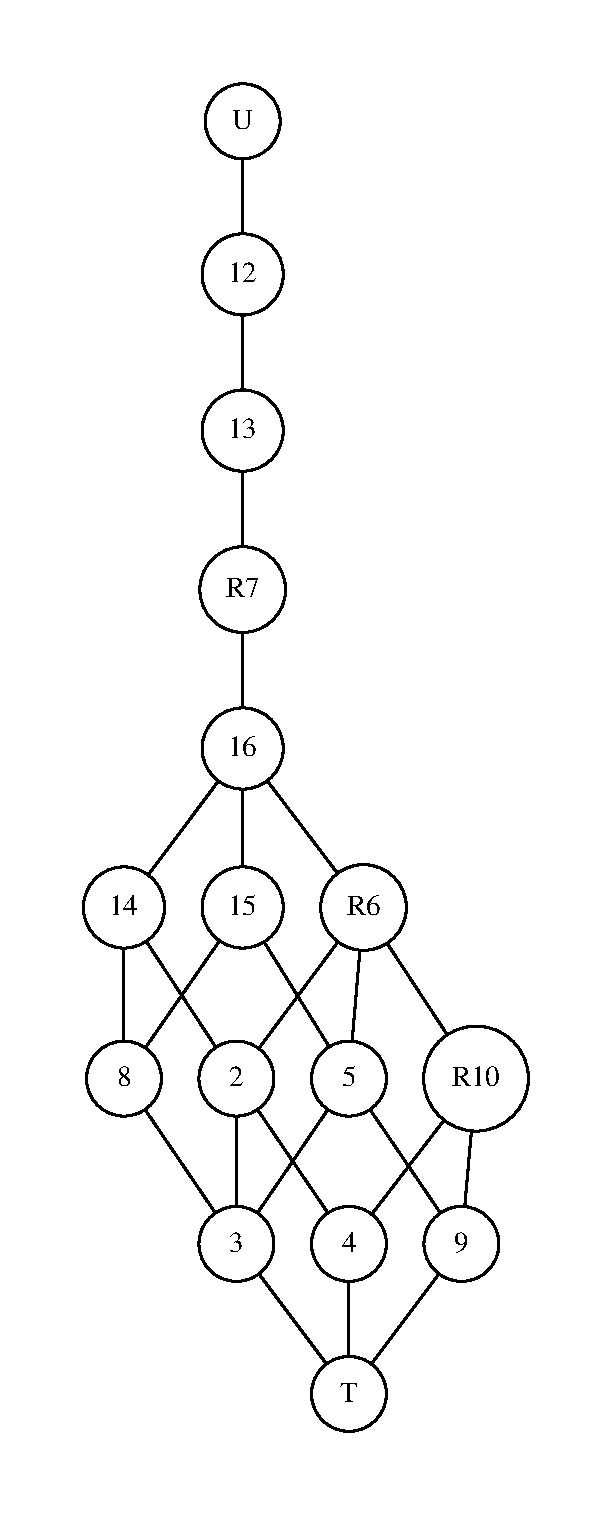
\includegraphics[scale=0.6]{pics/ch-motzkin/p3-lattice.pdf}
  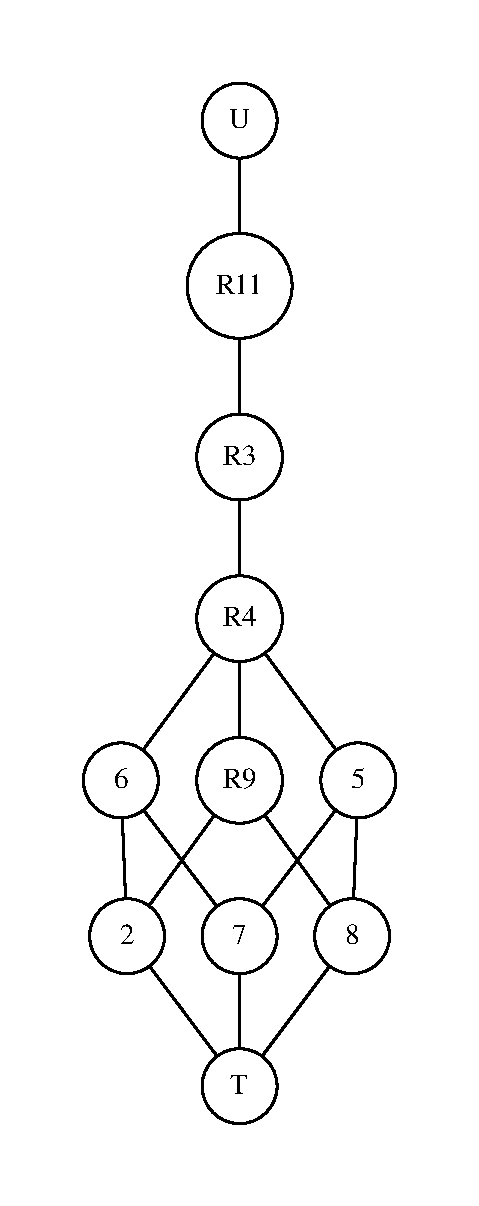
\includegraphics[scale=0.6]{pics/ch-motzkin/m4-lattice.pdf}
\begin{verbatim}
gap> Splash(DotString(LatticeOfCongruences(PartitionMonoid(3)),
>                     rec(info:=true)));
gap> Splash(DotString(LatticeOfCongruences(MotzkinMonoid(4)),
>                     rec(info:=true)));
\end{verbatim}
  \caption[Congruence lattices of $\Prt_3$ and $\Mot_4$ displayed using \GAP{}]
  {Congruence lattices of $\Prt_3$ (left) and $\Mot_4$ (right), as produced and
    displayed by the \Semigroups{} package for \GAP{}.  Here `T' represents the
    trivial congruence, `U' the universal congruence, and `R' a Rees congruence.
    Figures \ref{fig:pn-congs} and \ref{fig:mn-cong-lattice} illustrate these
    lattices with more meaningful labels}
  \label{fig:gap-lattices}
\end{figure}

With the rapidly increasing size of $\Prt_n$ (see Table \ref{tab:pn-size}) it
proved impractical to na\"ively calculate the congruence lattices beyond $n=4$,
but careful study of the lattices for small values of $n$, along with those
lattices computed for various submonoids of $\Prt_n$, yielded a general
classification of the congruence lattice of $\Prt_n$ for arbitrary $n$ (see
Figure \ref{fig:pn-congs}), along with a classification of the congruence
lattices of various important submonoids.  This classification is explained and
proven in \cite{ourpaper}, the paper upon which this chapter is based.
In this chapter, we will examine the structure of these congruence lattices.

As an author of \cite{ourpaper}, my particular focus was the Motzkin monoid
$\Mot_n$, which will be defined below.  The other authors on the paper used my
code for computing congruence lattices, as presented in Chapter
\ref{chap:lattice}, to study the congruences of $\Prt_n$, and they produced a
classification of its congruences.  I then modified and extended this work to
classify the congruences of the Motzkin monoid, and helped with general tasks
towards completing the paper.  As such, this chapter focuses on the Motzkin
monoid, only presenting the results for $\Prt_n$ and other monoids at the end.
Many of the results we describe here are contained in some form in
\cite{ourpaper}, and are included in this thesis with the kind permission of my
co-authors.

We will start with the definition of the Motzkin monoid $\Mot_n$, then describe
some preliminary theory, then describe the lattice of congruences of $\Mot_n$
(Theorem \ref{thm:mn-congs}), and finally give a brief description of how these
ideas can be extended to $\Prt_n$ and its other submonoids (Section
\ref{sec:motzkin-other}).

\section{The Motzkin monoid $\Mot_n$}
\label{sec:motzkin-monoid}
In order to define the Motzkin monoid, we must first define a \textit{planar}
bipartition.

\begin{definition}
  \label{def:planar}
  \index{planar bipartition}
  A bipartition of degree $n$ is called \textbf{planar} if, when represented in
  diagram form (see Section \ref{sec:bipartitions}),
  with the points $\{1, \ldots, n\}$ in left-to-right order forming the top of a
  rectangle,
  and the points $\{1', \ldots, n'\}$ in left-to-right order forming the bottom
  of the rectangle,
  with all edges contained inside the rectangle,
  it can be drawn without any edges crossing.
\end{definition}

\begin{example}
  Let $\alpha = \bipart{c|c|c|c}{2-4}{1,2 &3 &4 &5}{2,5 &1 &\mc2{c}{3,4}}$ and
  $\beta = \bipart{c|c|c|c}{3-4}{2 &5 &1,3 &4}{1 &3,4 &2 &5}$.  As can be seen
  in Figure \ref{fig:planar}, $\alpha$ is planar.  However, $\beta$ cannot be
  drawn inside the rectangle without the upper block $\{1,3\}$ crossing lines
  with the transversal $\{2, 1'\}$ -- hence, $\beta$ is not planar.
\end{example}

\begin{figure}[ht]
  \centering
  $$\alpha = \bipartdiag{\tc12\tv22\bC25 \bc34} \qquad
  \beta = \bipartdiag{\tc13 \tv21 \tv54\bc34}$$
  \caption{A planar and a non-planar bipartition}
  \label{fig:planar}
\end{figure}

We can now define the Motzkin monoid.

\begin{definition}
  \label{def:motzkin}
  \index{Motzkin monoid}
  \nomenclature[Mn]{$\Mot_n$}{Motzkin monoid}
  The \textbf{Motzkin monoid} $\Mot_n$ is the submonoid of $\Prt_n$ consisting
  of all planar bipartitions of degree $n$ in which every block has size $1$ or
  $2$.
\end{definition}

To see that this is indeed a monoid, we should observe that it is closed.  It is
easy to see that the product of two planar bipartitions is also planar, since a
double diagram as in Figure \ref{fig:bipartition-example} would contain no
crossing lines, and therefore would resolve to a product with no crossing lines.
It is also easy to see that if two bipartitions have no block larger than $2$,
their product also has no block larger than $2$: any transversal can only
contain one point in $\bn$ and one point in $\bn'$, so any transversal in the
product can only contain two points.  The upper and lower blocks of the product
are inherited from the original bipartitions, so they will not break the
condition either.

The Motzkin monoid $\Mot_n$ grows much slower than its parent $\Prt_n$, having
only $\sum_{k=0}^n \binom{2n}{2k}C_k$ elements
\citeoeis{A026945}, where $C_k$ is the $k$th
Catalan number.  Its size in comparison with $\Prt_n$ is shown in Table
\ref{tab:mn-size}.

\begin{table}[ht]
  \centering
  \renewcommand\arraystretch{1.0}
  \begin{tabular}{| r | r | r |}
    \hline
    $n$ & $|\Mot_n|$ & $|\Prt_n|$ \\
    \hline
     1 &           2 &                  2 \\
     2 &           9 &                 15 \\
     3 &          51 &                203 \\
     4 &         323 &              4 140 \\
     5 &       2 188 &            115 975 \\
     6 &      15 511 &          4 213 597 \\
     7 &     113 634 &        190 899 322 \\
     8 &     853 467 &     10 480 142 147 \\
     9 &   6 536 382 &    682 076 806 159 \\
    10 &  50 852 019 & 51 724 158 235 372 \\
    \hline
  \end{tabular}
  \renewcommand\arraystretch{0.7}
  \caption{Sizes of $\Mot_n$ and $\Prt_n$ for small values of $n$}
  \label{tab:mn-size}
\end{table}

The Motzkin monoid $\Mot_n$ shares a number of features with $\Prt_n$ -- indeed,
we will see later that its congruence lattice is very similar.  Like $\Prt_n$,
$\Mot_n$ is regular with a possible inverse given by the $^\star$
function. Another important similarity is in its Green's relations: consider the
following proposition, akin to Proposition \ref{prop:bipartition-greens}.

\begin{proposition}
  \label{prop:mn-greens}
  \nomenclature[Ik]{$I_k$}{Ideal of the Motzkin monoid $\Mot_n$}
  Let $\alpha$ and $\beta$ be bipartitions in $\Mot_n$.  The following hold:
  \begin{enumerate}[\rm(i)]
  \item $\alpha \RR \beta$ if and only if $\dom \alpha = \dom \beta$ and
    $\ker \alpha = \ker \beta$;
  \item $\alpha \LL \beta$ if and only if $\codom \alpha = \codom \beta$ and
    $\coker \alpha = \coker \beta$;
  \item $\alpha \JJ \beta$ if and only if $\rank \alpha = \rank \beta$;
  \item $J_\alpha \leq J_\beta$ if and only if $\rank \alpha \leq \rank \beta$;
  \item the ideals of $\Mot_n$ are precisely the sets
    $I_k=\{\alpha \in \Mot_n : \rank \alpha \leq k\}$ for
    $k \in \{0, \ldots, n\}$.
  \end{enumerate}
  \begin{proof}
    For (i) to (iii), see \cite[Theorem 2.4]{deg_motzkin}.  For (iv) and (v),
    see \cite[Proposition 2.6]{deg_motzkin}.
    % TODO? actually give the proof
  \end{proof}
\end{proposition}

This description of the Motzkin monoid's Green's relations, and its containment
of $\JJ$-classes and ideals, will help us greatly later on.  However, one
consequence of (i) and (ii) gives $\Mot_n$ a feature which $\Prt_n$ does not
share, namely the following corollary.

\begin{corollary}
  \label{cor:mn-h-trivial}
  The Motzkin monoid $\Mot_n$ is $\HH$-trivial.
  \begin{proof}
    Let $\alpha, \beta \in \Mot_n$ such that $\alpha \HH \beta$.  This tells us
    that $\alpha \LL \beta$ and $\alpha \RR \beta$, so by Proposition
    \ref{prop:mn-greens} parts (i) and (ii), we know that $\alpha$ and $\beta$
    share the same domain, kernel, codomain and cokernel.  The upper blocks and
    lower blocks of $\alpha$ and $\beta$ must certainly be the same, since they
    are just the blocks of the kernel and cokernel that do not lie in the domain
    or codomain.  The only choice is in the transversals: which blocks in the
    domain connect to which blocks in the codomain.  In $\Prt_n$ there are
    $(\rank \alpha)!$ ways of choosing this match-up; but in $\Mot_n$ there is
    only one way possible, since we cannot allow any lines in the diagram to
    cross.  Hence $\alpha = \beta$.
  \end{proof}
\end{corollary}

Finally, we will state one other feature of $\Mot_n$ that distinguishes it from
$\Prt_n$: an interesting property of its minimal ideal $I_0$.

\begin{lemma}
  \label{lem:i0-rect-band}
  Let $\alpha$ and $\beta$ be bipartitions in $I_0$, the minimal ideal of
  $\Mot_n$.  Then $\alpha \beta \alpha = \alpha$.
  % The product $\alpha\beta$ has the following proprties: $\ker\alpha\beta = \ker\alpha$,
  % $\coker\alpha\beta = \coker\beta$, and
  % $\dom\alpha\beta = \codom\alpha\beta = \varnothing$.
  \begin{proof}
    Since $\alpha$ has no transversals, $\alpha\beta\alpha$ also has no
    transversals.  The upper blocks of a product are equal to those of its first
    factor, the lower blocks to those of its last factor -- so $\alpha\beta\alpha$
    has the upper and lower blocks of $\alpha$.  Hence it equals $\alpha$.
  \end{proof}
\end{lemma}

The property described in the previous lemma implies that $I_0$ is a
\textit{rectangular band} (see Definition \ref{def:rectangular-band}).

\section{Lifted congruences}
\label{sec:motzkin-prelim}
We will now define some concepts which allow us to find certain
congruences in any semigroup: \textit{retractable ideals} (Definition
\ref{def:retractable-ideal}) and \textit{liftable congruences} (Definition
\ref{def:liftable-congruence}).  These constructions are new,
first appearing in \cite{ourpaper} to help describe some of the congruences on
$\Prt_n$ and its submonoids.  It will turn out that all non-Rees congruences
of $\Mot_n$ can be found using these two building blocks.

\begin{definition}
  \label{def:retractable-ideal}
  \index{retractable!ideal} \index{retraction}
  Let $S$ be a finite semigroup, with minimal ideal $M$.  An ideal $I$ of $S$ is
  called \textbf{retractable} if there exists some homomorphism $\phi: I \to M$
  such that $(m)\phi = m$ for all $m \in M$; we call $\phi$ a
  \textbf{retraction}.
\end{definition}

\begin{definition}
  \label{def:liftable-congruence}
  \index{liftable congruence}
  \nomenclature{$\sigma$}{Liftable congruence}
  Let $S$ be a finite semigroup, with minimal ideal $M$.  A congruence $\sigma$
  on $M$ is a \textbf{liftable congruence} of $S$ if either, and therefore both, of
  the following equivalent conditions are satisfied:
  \begin{enumerate}[\rm(i)]
  \item $\sigma \cup \Delta_S$ is a congruence on $S$;
  %\item there exists some congruence $\bar\sigma$ on $S$ such that
  %  $\sigma= \bar\sigma \cap (M \times M)$;
  \item $(ax,bx),(xa,xb) \in \sigma$ for all pairs $(a,b) \in \sigma$ and
    elements $x \in S$.
  \end{enumerate}
\end{definition}

To see that the two conditions in the last definition are equivalent, assume we
have $S$, $M$ and $\sigma$ such that (i) is satisfied.  Now let
$(a,b) \in \sigma$ and $x \in S$ be arbitrary.  Since $\sigma \cup \Delta_S$ is
a congruence and $(a,b) \in \sigma \cup \Delta_S$, we must have
$(ax,bx) \in \sigma \cup \Delta_S$.  If $(ax,bx) \in \Delta_S$ then $ax=bx$, and
since $M$ is an ideal we must have both $ax$ and $bx$ in $M$; hence $(ax,bx)$ is
a reflexive pair and lies in the congruence $\sigma$.  Hence $(ax,bx)$ is in
$\sigma$, and by a similar argument, so is $(xa,xb)$, so we have (ii).

Conversely, assume that (ii) holds, let $(a,b) \in \sigma \cup \Delta_S$, and
let $x \in S$.  If $(a,b) \in \Delta_S$ then $a=b$, and so $ax=bx$ and $xa=xb$.
Otherwise, $(a,b) \in \sigma$ and by (ii) we have $(ax,bx),(xa,xb) \in \sigma$.
In either case, we have $(ax,bx),(xa,xb) \in \sigma \cup \Delta_S$, and so we
have (i).

In order to use these building blocks to produce new congruences, we first need
to establish some results about them.  Note that, since $\Mot_n$ is finite, it
must have a minimal ideal.  More specifically, the minimal ideal of $\Mot_n$ is
given by $I_0 = \{\alpha \in \Mot_n : \rank \alpha = 0\}$ (see Proposition
\ref{prop:mn-greens}).  The following lemma will be used at various times
throughout this chapter.

\begin{lemma}
  \label{lem:retract-aux}
  Let $S$ be a finite semigroup with minimal ideal $M$, and let $I$ be
  an ideal of $S$.  If $I$ is retractable and $\phi$ is a
  retraction from $I$ to $M$, then $(sxt)\phi=s \cdot (x)\phi \cdot t$ for all
  elements $x \in I$ and all $s,t\in S^1$.
  \begin{proof}
    Since $S$ is a finite semigroup, we know that its minimal ideal $M$ is
    regular, by \cite[Proposition 3.1.4]{howie}.  Hence
    any element $m \in M$ has an inverse $m' \in M$.  Since $(mm')m = m$, we
    have a left identity for $m$; and since $m(m'm) = m$, we also have a right
    identity.  Let $e$ be a right identity for $(x)\phi$, so that
    $(x)\phi \cdot e = (x)\phi$.  Since $\phi$ is a retraction and
    $e, xe \in M$, we have
    $$(x)\phi=(x)\phi \cdot e = (x)\phi \cdot (e)\phi = (xe)\phi = xe,$$
    so $(x)\phi = xe$.
    Now let $f$ be a left identity for $(sx)\phi$; we also
    have
    \begin{align*}
      (sx)\phi \cdot e & = f \cdot (sx)\phi \cdot e \\
      & = (f)\phi \cdot (sx)\phi \cdot e \\
      & = (fsx)\phi \cdot e \\
      & = (fs)\phi \cdot (x)\phi \cdot e \\
      & = (fs)\phi \cdot (x)\phi \\
      & = (fsx)\phi \\
      & = (f)\phi \cdot (sx)\phi \\
      & = f \cdot (sx)\phi \\
      & = (sx)\phi,
    \end{align*}
    which shows that $e$ is a right identity for $(sx)\phi$ as well as for
    $(x)\phi$.  Hence we have
    $$s \cdot (x)\phi = s \cdot xe = (sxe)\phi = (sx)\phi \cdot (e)\phi =
    (sx)\phi \cdot e = (sx)\phi,$$ i.e.~$\phi$ respects left multiplication; a
    symmetric argument gives $(xt)\phi = (x)\phi \cdot t$, i.e.~$\phi$ respects
    right multiplication too.  Finally we can combine these to give
    $(sxt)\phi = (sx)\phi \cdot t = s \cdot (x)\phi \cdot t$, as required.
  \end{proof}
\end{lemma}

The previous lemma gives rise to an important corollary which we can use later
when we combine retractable ideals with liftable congruences.

\begin{corollary}
  \label{cor:retract-unique}
  Let $S$ be a finite semigroup, with minimal ideal $M$.  If $I$ is a
  retractable ideal of $S$, then the retraction $\phi:I \to M$ is unique.
  \begin{proof}
    Let $\phi$ and $\psi$ be retractions from $I$ to $M$.  Let $x \in I$,
    and let $e_l$ and $e_r$ be left and right identities for $(x)\phi$.  By
    Lemma \ref{lem:retract-aux}, we have
    $$(x)\phi
    = e_l \cdot (x)\phi
    = (e_lx)\phi
    = e_lx
    = (e_lx)\psi
    = e_l \cdot (x)\psi,$$
    so $(x)\phi = e_l \cdot (x)\psi$.  Similarly,
    $$(x)\psi
    = (x)\psi \cdot e_r
    = (xe_r)\psi
    = xe_r
    = (xe_r)\phi
    = (x)\phi \cdot e_r,$$
    so $(x)\psi = (x)\phi \cdot e_r$.  But then
    $$(x)\phi
    = e_l \cdot (x)\psi
    = e_l \cdot (x)\phi \cdot e_r
    = (x)\phi \cdot e_r
    = (x)\psi,$$
    so $\phi = \psi$.
  \end{proof}
\end{corollary}

The effect of Corollary \ref{cor:retract-unique} is that, for a finite
semigroup, regular minimal ideal, we can talk about \textit{the} retraction of a
retractable ideal without any loss of generality.  We can now use our two
building blocks to produce a new congruence: a \textit{lifted congruence}.

\begin{definition}
  \label{def:lifted-congruence}
  \index{lifted congruence}
  \nomenclature{$\zeta_{I,\sigma}$}{Lifted congruence}
  Let $S$ be a semigroup with minimal ideal $M$, let $I$ be a retractable
  ideal of $S$, and let $\sigma$ be a liftable congruence of $S$.  We associate
  to the pair $(I,\sigma)$ the relation
  $$\zeta_{I,\sigma} = \Big\{(x,y) \in I \times I :
  \big((x)\phi,(y)\phi\big) \in \sigma\Big\} \cup \Delta_S,$$
  where $\phi$ is the unique retraction from $I$ to $M$.
  We call $\zeta_{I,\sigma}$ the \textbf{lifted congruence} of $(I,\sigma)$.
\end{definition}

In order to justify the name \textit{lifted congruence}, we require the
following proposition.

\begin{theorem}
  \label{thm:lifted-congruence}
  The relation $\zeta_{I,\sigma}$ in Definition \ref{def:lifted-congruence} is a
  congruence on $S$.
  \begin{proof}
    For conciseness, let us refer to $\zeta_{I,\sigma}$ as $\zeta$.  Let $(x,y)$
    be a pair in $\zeta$ and let $s \in S$.  To show $\zeta$ is a congruence, we
    must show that $(sx,sy)$ and $(xs,ys)$ both lie in $\zeta$.  If
    $(x,y) \in \Delta_S$, this is certainly true.  Otherwise, we have
    $x, y \in I$ and $\big((x)\phi, (y)\phi\big) \in \sigma$.  Since $I$ is an
    ideal, we certainly have $xs,ys\in I$.  Now by Definition
    \ref{def:liftable-congruence} part (ii), and by Lemma
    \ref{lem:retract-aux}, we have
    $$\big(s \cdot (x)\phi, s \cdot (y)\phi\big)
    = \big((sx)\phi, (sy)\phi\big) \in \sigma,$$
    so $(sx, sy) \in \zeta$.  A symmetric argument gives us $(xs,ys) \in \zeta$.
  \end{proof}
\end{theorem}

This construction now gives us a usable source of congruences.  All that is
required is to find some liftable congruences and retractable ideals of a
semigroup, and a number of new congruences can be described.  It turns out that
this is an excellent source of congruences for $\Mot_n$, yielding every non-Rees
congruence on the semigroup, as we will see later.

\section{Congruence lattice of $\Mot_n$}
\label{sec:motzkin-congs}

% Rees congruences

We can now apply the general theory of Section \ref{sec:motzkin-prelim} to the
Motzkin monoid, in order to find its congruences.  First, let us mention the
easiest congruences to describe -- the Rees congruences (Definition
\ref{def:rees-congruence}).

\begin{proposition}
  \label{prop:motzkin-rees}
  \nomenclature[Rk]{$R_k$}{Rees congruence of the Motzkin monoid $\Mot_n$}
  The Rees congruences of $\Mot_n$ are the relations
  $$R_k = \{(x,y) \in \Mot_n \times \Mot_n : \rank x, \rank y \leq k\} \cup
  \Delta_{\Mot_n},$$
  for $k \in \{0, \ldots, n\}$.
  \begin{proof}
    This follows immediately from the description of the ideals of $\Mot_n$ in
    Proposition \ref{prop:mn-greens} part (v).
  \end{proof}
\end{proposition}

We will refer to these congruences by the name $R_k$ for the rest of this
chapter.  We will soon see that $R_0$ and $R_1$ are in fact lifted congruences.
The higher Rees congruences are not lifted congruences, as we will see in
Corollary \ref{cor:rk-not-lifted}.  Next, we will describe some other lifted
congruences, by identifying some liftable congruences and retractions in
$\Mot_n$ to use as building blocks.

% L,R,H,Delta,Univ are liftable congs: lambda, rho, mu, eta, R
First, recall that $I_0 = \{\alpha \in \Mot_n : \rank \alpha = 0\}$ is the
minimal ideal of $\Mot_n$.  Let us denote by $\LL^{I_0}$ and $\RR^{I_0}$ the $\LL$- and
$\RR$-relations of $\Mot_n$ restricted to $I_0$, and let $\Delta_{I_0}$ and
$\nabla_{I_0}$ be the trivial and universal congruences respectively on $I_0$.
\nomenclature[Lc0]{$\LL^{I_0}$}{Green's $\LL$-relation retricted to the ideal $I_0$}
\nomenclature[Raa0]{$\RR^{I_0}$}{Green's $\RR$-relation retricted to the ideal $I_0$}

\begin{proposition}
  The relations $\Delta_{I_0}$, $\lL^{I_0}$, $\rR^{I_0}$ and $\nabla_{I_0}$ are all
  liftable congruences of $\Mot_n$.
  \begin{proof}
    Since $I_0$ is a semigroup, $\Delta_{I_0}$ and $\nabla_{I_0}$ are certainly
    congruences of $I_0$; and both satisfy Definition
    \ref{def:liftable-congruence}(i), since their unions with $\Delta_{\Mot_n}$
    are the congruences $\Delta_{\Mot_n}$ and $R_0$ respectively.

    To see that $\lL^{I_0}$ is a liftable congruence, consider Definition
    \ref{def:liftable-congruence}(ii); let $(a,b) \in \lL^{I_0}$ and
    $x \in \Mot_n$.  Since $I_0$ is the minimal ideal, we certainly have
    $xa,xb,ax,bx \in I_0$; and since $\LL$ is a right congruence on $\Mot_n$
    (see Proposition \ref{prop:greens-as-congs}) we have $(ax,bx) \in \lL$ and
    therefore $(ax,bx) \in \lL^{I_0}$.  By Lemma \ref{lem:i0-rect-band} we also have
    $a(xa) = a$, so $xa \LL a$ and similarly $xb \LL b$.  This means that
    $xa \LL a \LL b \LL xb$, so $(xa, xb) \in \lL^{I_0}$.  Hence $\lL^{I_0}$ is a
    liftable congruence of $\Mot_n$, and by a similar argument, so is $\rR^{I_0}$.
  \end{proof}
\end{proposition}

% ^ notation
Now that we have some liftable congruences, we also want some retractable ideals
in order to form lifted congruences.  The following construction establishes one
such ideal.

\begin{definition}
  \label{def:mn-hat}
  \nomenclature[^]{$\widehat{\phantom\alpha}$}{Bipartition of rank $0$ with this
    kernel and cokernel}
  If $\alpha$ is a bipartition, then $\widehat\alpha$ is the unique bipartition
  of rank $0$ with the same kernel and cokernel as $\alpha$.
\end{definition}

The element $\widehat\alpha$ can be computed easily from $\alpha$: each
transversal is split into an upper block (the points in $\bn$) and a lower block
(the points in $\bn'$) and nothing else is changed.  If we have a diagram for
$\alpha$, drawn in the standard way described after Example
\ref{ex:bipartition}, then we simply remove any lines crossing the diagram.  If
we are using two-row notation, we can simply draw a horizontal line between the
two rows.  See Figure \ref{fig:hat} for an example.  Note that $\widehat\alpha =
\alpha$ for all $\alpha \in I_0$.

\begin{figure}[ht]
  \centering
  $$\alpha = \big\{
    \{1\}, \{2,1'\}, \{3,5'\}, \{4,5\}, \{2',4'\}, \{3'\}
  \big\}$$
  $$\widehat\alpha = \big\{
    \{1\}, \{2\}, \{3\}, \{4,5\}, \{1'\}, \{2',4'\}, \{3'\}, \{5'\}
  \big\}$$
  $$\alpha = \bipartdiag{\tv21 \tv35 \tc45 \bc24} \quad
  \widehat\alpha = \bipartdiag{\tc45 \bc24}$$
  $$\alpha = \bipart{c|c|c|c}{3-4}{2 & 3 & 1 & 4,5}{1 & 5 & 2,4 & 3} \quad
  \widehat\alpha = \bipart{c|c|c|c}{1-4}{2 & 3 & 1 & 4,5}{1 & 5 & 2,4 & 3}$$
  \caption{Computing $\widehat\alpha$ from $\alpha$}
  \label{fig:hat}
\end{figure}

% Show ^:I1->I0 is a retraction
\begin{proposition}
  \label{prop:hat-retraction}
  The map $\phi: I_1 \to I_0$ defined by $\alpha \mapsto \widehat\alpha$ is a
  retraction.  Hence, $I_1$ is a retractable ideal.
  \begin{proof}
    Since $\widehat\alpha = \alpha$ for $\alpha \in I_0$, we can see that $\phi$
    satisfies the condition $(m)\phi = m$ from Definition
    \ref{def:retractable-ideal}.  Hence we only need to show that $\phi$ is a
    homomorphism. Let
    $\alpha,\beta \in I_1$, and we will try to prove that
    $\widehat{\alpha\beta} = \widehat\alpha \widehat\beta$.  If both $\alpha$
    and $\beta$ have rank $0$ then
    $\widehat{\alpha\beta} = \alpha\beta = \widehat\alpha \widehat\beta$.  On
    the other hand, if at least one of $\alpha$ and $\beta$ has rank $1$ (without
    loss of generality, $\alpha$) then we may write
    $\alpha = \bipart{c|c|c|c}{2-4}{A_0&A_1&\ldots&A_r}{B_0&B_1&\ldots&B_s}$ and
    $\beta = \bipart{c|c|c|c}{2-4}{C_0&C_1&\ldots&C_t}{D_0&D_1&\ldots&D_u}$ or
    $\beta = \bipart{c|c|c|c}{1-4}{C_0&C_1&\ldots&C_t}{D_0&D_1&\ldots&D_u}$.
    This gives us
    $\alpha\beta =
    \bipart{c|c|c|c}{2-4}{A_0&A_1&\ldots&A_r}{D_0&D_1&\ldots&D_u}$ or
    $\alpha\beta =
    \bipart{c|c|c|c}{1-4}{A_0&A_1&\ldots&A_r}{D_0&D_1&\ldots&D_u}$.  Applying
    $\phi$ gives us
    $\widehat\alpha =
    \bipart{c|c|c|c}{1-4}{A_0&A_1&\ldots&A_r}{B_0&B_1&\ldots&B_s}$,
    $\widehat\beta =
    \bipart{c|c|c|c}{1-4}{C_0&C_1&\ldots&C_t}{D_0&D_1&\ldots&D_u}$, and finally
    $\widehat{\alpha\beta} =
    \bipart{c|c|c|c}{1-4}{A_0&A_1&\ldots&A_r}{D_0&D_1&\ldots&D_u} =
    \widehat\alpha \widehat\beta$, so $\phi$ is a homomorphism.
  \end{proof}
\end{proposition}

This gives us a retractable ideal $I_1$, with a retraction
$\alpha \mapsto \widehat\alpha$.  It is also trivial to see that $I_0$ itself is
retractable, with retraction $\alpha \mapsto \alpha$, the identity map.  Since
the minimal ideal $\I_0$ is regular, Corollary \ref{cor:retract-unique} shows
that these retractions are unique.

% Describe the congruences:
% mu0, lam0, rho0, R0,
% mu1, lam1, rho1, R1,
% R2 ... Rn
We now have four liftable congruences $\left\{\Delta_{I_0}, \lL^{I_0}, \rR^{I_0}, \nabla_{I_0}\right\}$ and
two retractable ideals $\{I_0, I_1\}$, giving rise to $4 \times 2 = 8$ lifted
congruences by Definition \ref{def:lifted-congruence} and Theorem
\ref{thm:lifted-congruence}.  The congruences lifted from $\nabla_{I_0}$ are
observed to be equal to the Rees congruences $R_0$ and $R_1$, while those lifted
from $\Delta_{I_0}$, $\lL^{I_0}$ and $\rR^{I_0}$ are named with appropriate Greek symbols,
as follows:
\begin{align*}
  \delta_0 &= \zeta_{I_0,\Delta_{I_0}}
  = \{(\alpha,\beta) \in I_0 \times I_0 :
    (\alpha, \beta) \in \Delta_{I_0}\} \cup \Delta_{\Mot_n}, \\
  \delta_1 &= \zeta_{I_1,\Delta_{I_0}}
  = \{(\alpha,\beta) \in I_1 \times I_1 :
    (\widehat\alpha, \widehat\beta) \in \Delta_{I_0}\} \cup \Delta_{\Mot_n}, \\
  \lambda_0 &=\zeta_{I_0,\lL^{I_0}}
  = \{(\alpha,\beta) \in I_0 \times I_0 :
    (\alpha, \beta) \in \lL^{I_0}\} \cup \Delta_{\Mot_n}, \\
  \lambda_1 &= \zeta_{I_1,\lL^{I_0}}
  = \{(\alpha,\beta) \in I_1 \times I_1 :
    (\widehat\alpha, \widehat\beta) \in \lL^{I_0}\} \cup \Delta_{\Mot_n}, \\
  \rho_0 &= \zeta_{I_0,\rR^{I_0}}
  = \{(\alpha,\beta) \in I_0 \times I_0 :
    (\alpha, \beta) \in \rR^{I_0}\} \cup \Delta_{\Mot_n}, \\
  \rho_1 &= \zeta_{I_1,\rR^{I_0}}
  = \{(\alpha,\beta) \in I_1 \times I_1 :
    (\widehat\alpha, \widehat\beta) \in \rR^{I_0}\} \cup \Delta_{\Mot_n}, \\
  R_0 &= \zeta_{I_0,\nabla_{I_0}}
  = \{(\alpha,\beta) \in I_0 \times I_0 :
    (\alpha, \beta) \in \nabla_{I_0}\} \cup \Delta_{\Mot_n}, \\
  R_1 &= \zeta_{I_1,\nabla_{I_0}}
  = \{(\alpha,\beta) \in I_1 \times I_1 :
    (\widehat\alpha, \widehat\beta) \in \nabla_{I_0}\} \cup \Delta_{\Mot_n}.
\end{align*}

This naming convention is summarised in Table \ref{tab:mn-lifted-congruences}.

\begin{table}[ht]
  \centering
  \renewcommand\arraystretch{1.3}
  \begin{tabular}[ht]{| c | c | c |}
    \cline{2-3}
    \mc1{c|}{} & $I_0$ & $I_1$ \\ \hline
    $\Delta_{I_0}$ & $\delta_0$ & $\delta_1$ \\ \hline
    $\lL^{I_0}$ & $\lambda_0$ & $\lambda_1$ \\ \hline
    $\rR^{I_0}$ & $\rho_0$ & $\rho_1$ \\ \hline
    $\nabla_{I_0}$ & $R_0$ & $R_1$ \\ \hline
  \end{tabular}
  \caption{Lifted congruences of $\Mot_n$}
  \label{tab:mn-lifted-congruences}
\end{table}

Interpreting these statements along with the use of Proposition
\ref{prop:mn-greens} gives the following characterisation of the lifted
congruences in terms of a bipartition's rank, kernel and cokernel.

\begin{proposition}
  \label{prop:mn-cong-char}
  The lifted congruences of $\Mot_n$ can be characterised in the following way,
  where $(\alpha, \beta) \in \Mot_n \times \Mot_n$:
  \begin{align*}
    \delta_0 &= \Delta_{\Mot_n}, \\
    \delta_1 &= \{(\alpha,\beta) :
                  \rank\alpha,\rank\beta \leq 1,
                  \ker\alpha = \ker\beta,
                  \coker\alpha = \coker\beta\} \cup \Delta_{\Mot_n}, \\
    \lambda_0 &= \{(\alpha,\beta) :
                   \rank\alpha,\rank\beta = 0,
                   \coker\alpha = \coker\beta\} \cup \Delta_{\Mot_n}, \\
    \lambda_1 &= \{(\alpha,\beta) :
                   \rank\alpha,\rank\beta \leq 1,
                   \coker\alpha = \coker\beta\} \cup \Delta_{\Mot_n}, \\
    \rho_0 &= \{(\alpha,\beta) :
                \rank\alpha,\rank\beta = 0,
                \ker\alpha = \ker\beta\} \cup \Delta_{\Mot_n}, \\
    \rho_1 &= \{(\alpha,\beta) :
                \rank\alpha,\rank\beta \leq 1,
                \ker\alpha = \ker\beta\} \cup \Delta_{\Mot_n}, \\
    R_0 &= \{(\alpha,\beta) :
             \rank\alpha,\rank\beta = 0\} \cup \Delta_{\Mot_n}, \\
    R_1 &= \{(\alpha,\beta) :
             \rank\alpha,\rank\beta \leq 1\} \cup \Delta_{\Mot_n}.
  \end{align*}
\end{proposition}
These characterisations will help us later when we consider generating pairs for
the congruences.

We are now ready to state the main theorem of this chapter, giving a full
description of the congruence lattice of $\Mot_n$.  Much of the work to prove
this has already been done, and the rest of this section will be devoted to
completing the proof.  Note that our main theorem requires $n \geq 2$; if
$n = 1$ then $\Mot_n$ has only $2$ elements, and its congruences are only
$\Delta_{\Mot_n}$ and $\nabla_{\Mot_n}$.

\begin{theorem}
  \label{thm:mn-congs}
  Let $\Mot_n$ be the Motzkin monoid, with $n \geq 2$.  The following hold:
  \begin{enumerate}[\rm(i)]
  \item The congruences of $\Mot_n$ are precisely
    $\{\delta_0, \delta_1, \lambda_0, \lambda_1, \rho_0, \rho_1, R_0, R_1,
    \ldots, R_n\}$;
  \item The congruence lattice of $\Mot_n$ is shown in Figure
    \ref{fig:mn-cong-lattice};
  \item Every congruence of $\Mot_n$ is principal;
  \item Each congruence $\sigma$ of $\Mot_n$ is generated by any single pair
    from $\sigma$ not contained in any congruence below $\sigma$ in the
    congruence lattice.
  \end{enumerate}
\end{theorem}

% Show the lattice
\begin{figure}[ht]
  \centering
  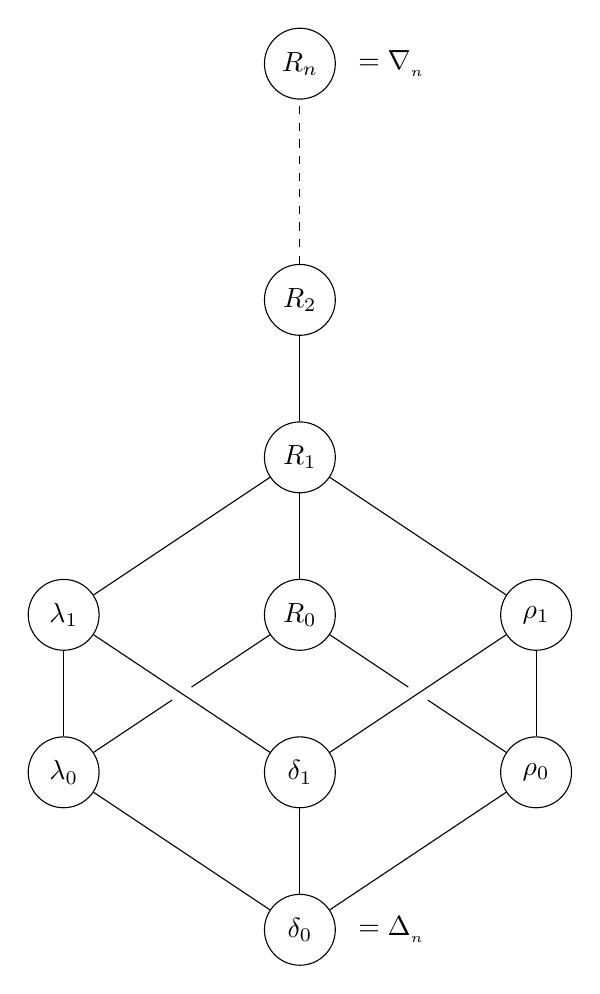
\begin{tikzpicture}
    [cong/.style={circle, minimum size=0.9cm, draw}]
    \node[cong] (Rn) at ( 0,13) {$R_n$};
    \node[cong] (R2) at ( 0,10) {$R_2$};
    \node[cong] (R1) at ( 0, 8) {$R_1$};
    \node[cong] (l1) at (-3, 6) {$\lambda_1$};
    \node[cong] (R0) at ( 0, 6) {$R_0$};
    \node[cong] (r1) at ( 3, 6) {$\rho_1$};
    \node[cong] (l0) at (-3, 4) {$\lambda_0$};
    \node[cong] (d1) at ( 0, 4) {$\delta_1$};
    \node[cong] (r0) at ( 3, 4) {$\rho_0$};
    \node[cong] (d0) at ( 0, 2) {$\delta_0$};
    \node at (1.17,13) {$=\nabla_{\Mot_n}$};
    \node at (1.17, 2) {$=\Delta_{\Mot_n}$};
    \draw (d0)--(l0) (d0)--(r0) (l0)--(R0) (r0)--(R0);
    \fill[white] (-1.5,5)circle(.15) (+1.5,5)circle(.15);
    \draw (d0)--(d1) (l0)--(l1) (r0)--(r1) (R0)--(R1);
    \draw (d1)--(l1) (d1)--(r1) (l1)--(R1) (r1)--(R1);
    \draw (R1)--(R2);
    \draw[dashed] (R2)--(Rn);
  \end{tikzpicture}
  \caption[Congruence lattice of $\Mot_n$]{Congruence lattice of $\Mot_n$ (Hasse diagram)}
  \label{fig:mn-cong-lattice}
\end{figure}

The remainder of this section serves to prove Theorem \ref{thm:mn-congs}, as
follows.  Let $\Gamma$ be the set of relations stated in (i).  That the
relations in $\Gamma$ are congruences has already been established.  In order to
see that these congruences are all distinct, we analyse the possible generating
pairs of each congruence in Lemmas \ref{lem:low-genpairs},
\ref{lem:high-genpairs} and \ref{lem:rees-genpairs}.  These results, which are
summarised in Table \ref{tab:mn-genpairs}, exhaust all pairs in
$\Mot_n \times \Mot_n$ and all congruences in $\Gamma$, proving that all the
congruences in $\Gamma$ are principal, and that there are no other principal
congruences.  Next we consider the joins of these congruences in Lemmas
\ref{lem:mn-lattice-intra} and \ref{lem:mn-lattice-inter}.  These show that the
congruences join together as in Figure \ref{fig:mn-cong-lattice}, and therefore
that $\Gamma$ is closed under taking joins.  Since any congruence is a join of
principal congruences, this proves that $\Mot_n$ has no congruences other than
those in $\Gamma$.  This completes the proof of (i), (ii) and (iii), and
inspection of Table \ref{tab:mn-genpairs} establishes (iv).

% Proof of exhaustion: table of generating pairs, with references to
% propositions
We will now state the lemmas required to complete the
proof of Theorem \ref{thm:mn-congs}.  Firstly, we will focus on generating
pairs: we will consider a pair $(\alpha, \beta)$ and decide which principal
congruence it generates.  Our findings are summarised in Table
\ref{tab:mn-genpairs}.

\begin{table}[ht]
  \renewcommand\arraystretch{1.0}
  \centering
  \begin{tabular}{| c | l | l |}
    \hline
    $(\alpha,\beta)^\sharp$ & $(\alpha,\beta) \in$ & Reference \\
    \hline
    $\delta_0$   & $\delta_0$
                 & Trivial                             \\
    $\delta_1$   & $\delta_1 \setminus \delta_0$
                 & Lemma \ref{lem:low-genpairs}(iii)  \\
    $\lambda_0$  & $\lambda_0 \setminus \delta_0$
                 & Lemma \ref{lem:low-genpairs}(i)    \\
    $\lambda_1$  & $\lambda_1 \setminus (\lambda_0 \cup \delta_1)$
                 & Lemma \ref{lem:high-genpairs}(i)   \\
    $\rho_0$     & $\rho_0 \setminus \delta_0$
                 & Lemma \ref{lem:low-genpairs}(ii)   \\
    $\rho_1$     & $\rho_1 \setminus (\rho_0 \cup \delta_1)$
                 & Lemma \ref{lem:high-genpairs}(ii)  \\
    $R_0$        & $R_0 \setminus (\lambda_0 \cup \rho_0)$
                 & Lemma \ref{lem:high-genpairs}(iii) \\
    $R_1$        & $R_1 \setminus (\lambda_1 \cup \rho_1 \cup R_0)$
                 & Lemma \ref{lem:high-genpairs}(iv)  \\
    $R_{k \geq 2}$ & $R_k \setminus R_{k-1}$
                 & Lemma \ref{lem:rees-genpairs}       \\
    \hline
  \end{tabular}
  \caption{Generating pairs for each congruence on $\Mot_n$}
  \label{tab:mn-genpairs}
\end{table}

\begin{lemma}
  \label{lem:low-genpairs}
  Let $\alpha,\beta \in \Mot_n$.  The following hold:
  \begin{enumerate}[\rm(i)]
  \item $\lambda_0 = (\alpha, \beta)^\sharp$ if and only if
    $(\alpha,\beta) \in \lambda_0 \setminus \Delta$;
  \item $\rho_0 = (\alpha, \beta)^\sharp$ if and only if
    $(\alpha,\beta) \in \rho_0 \setminus \Delta$;
  \item $\delta_1 = (\alpha, \beta)^\sharp$ if and only if
    $(\alpha,\beta) \in \delta_1 \setminus \Delta$.
  \end{enumerate}
  \begin{proof}
    In each statement, the ``only if'' part is obvious.  We will prove (i) and
    observe that (ii) follows from a symmetric argument.  Then we will prove
    (iii) separately. % TODO? make this precise, with "duality"

    For (i), let $(\alpha, \beta) \in \lambda_0 \setminus \Delta$, and let
    $\sigma = (\alpha, \beta)^\sharp$.  Since $\lambda_0$ is a congruence, we
    clearly have $\sigma \subseteq \lambda_0$; hence we have only to prove that
    $\lambda_0 \subseteq \sigma$.  First we require a special construction: if
    $\gamma \in I_0$, let $\gamma'$ be the unique bipartition in $I_0$ with
    trivial kernel and $\coker\gamma' = \coker\gamma$.  We claim that
    $(\gamma, \gamma') \in \sigma$ for any such $\gamma$.  This claim is proven
    by descending induction on $r$, the number of kernel-classes of $\gamma$: if
    $r = n$ (trivial kernel) then $\gamma = \gamma'$ and we are done.  Otherwise
    we have $r \leq n-1$, and we write
    $\gamma = \bipart{c|c|c}{1-3}{A_1&\ldots&A_r}{B_1&\ldots&B_s}$.  Since
    $(\alpha,\beta) \in \lambda_0 \setminus \Delta$, Propisition
    \ref{prop:mn-cong-char} gives us $\rank\alpha = \rank\beta = 0$ and
    $\coker\alpha = \coker\beta$, but since $\alpha \neq \beta$ we must have
    $\ker\alpha \neq \ker\beta$.  Swapping $\alpha$ and $\beta$ if necessary,
    let us assume there exists some $(i,j) \in \ker\alpha \setminus \ker\beta$,
    and without loss of generality, assume $i < j$.  We will write
    $\bn \setminus \{i,j\}$ as $\{k_1, \ldots, k_{n-2}\}$.  Since $r \leq n-1$
    there exists some kernel block of $\gamma$ with 2 elements; let $m$
    be the lowest point in $\bn$ in a non-trivial kernel block, and without loss
    of generality, let us assume $m$ lies in $A_1$.  We can now define the
    bipartition $\tau = \bipart{c|c|c|c|c}{3-5}
    {m & p & A_2 & \ldots & A_r}
    {i & j & k_1 & \ldots & k_{n-2}}$, 
    where $A_1 = \{m, p\}$.
    We observe that $\tau \alpha \gamma = \gamma = \bipart{c|c|c|c|c}{1-5}
    {\mc2{c|}{m,p} & A_2 & \ldots & A_r}
    {B_1 & B_2 & B_3 & \ldots & B_s}$ and
    $\tau \beta \gamma = \bipart{c|c|c|c|c}{1-5}
    {m & p & A_2 & \ldots & A_r}
    {B_1 & B_2 & B_3 & \ldots & B_s}$.
    Since $\sigma$ is left- and right-compatible, we have
    $\gamma = \tau\alpha\gamma \mathrel\sigma \tau\beta\gamma$.  Hence $\gamma$
    is $\sigma$-related to $\tau\beta\gamma$, a bipartition with rank $0$, the
    same cokernel as $\gamma$, and $r+1$ kernel classes.  Applying the same
    process inductively, with $\tau\beta\gamma$ in place of $\gamma$, implies a
    chain of $\sigma$-relations which relate $\gamma$ to a bipartition with rank
    $0$, the same cokernel as $\gamma$, and $n$ kernel classes -- that is,
    $\gamma'$.  This proves the claim that $(\gamma, \gamma') \in \sigma$.

    To return to the proof that $\lambda_0 \subseteq \sigma$, let
    $(\mu, \nu) \in \lambda_0$ be arbitrary.  If $\mu = \nu$ then certainly
    $(\mu, \nu) \in \sigma$, so let us assume $\mu \neq \nu$.  By Proposition
    \ref{prop:mn-cong-char} we must have $\rank\mu = \rank\nu = 0$ and
    $\coker\mu = \coker\nu$, so we have $\mu' = \nu'$.  Hence, by the above
    claim, we have $\mu \mathrel\sigma \mu' = \nu' \mathrel\sigma \nu$,
    so $(\mu, \nu) \in \sigma$, and (i) is complete.  Observe that (ii) follows
    by a similar argument.

    To prove (iii), let $(\alpha,\beta)\in\delta_1\setminus\Delta$ as stated,
    and let $\sigma = (\alpha,\beta)^\sharp$.  Clearly
    $\sigma \subseteq \delta_1$; it remains to prove that
    $\delta_1 \subseteq \sigma$.  Since
    $(\alpha,\beta) \in \delta_1 \setminus \Delta$, $\alpha$ and $\beta$ must
    each have rank $0$ or $1$, and have the same kernel and
    cokernel, but be distinct.  Since there is only one bipartition of rank $0$
    with a given kernel and cokernel, they cannot both have rank $0$.  Hence,
    swapping $\alpha$ and $\beta$ if necessary, we may assume that
    $\rank(\alpha)=1$, with transversal $\{i,j'\}$, and we can write
    $\alpha=\bipart{c|c|c|c}{2-4}
    {i & A_1 & \cdots & A_r}{j & B_1 & \cdots & B_s}$.
    Then $\beta$ has one of the following four forms, where without loss of
    generality, additional labelled elements are assumed to be from $A_1$:
    \begin{enumerate}[\rm(a)]
    \item $\beta = \bipart{c|c|c|c|c}{1-5}
      {i & A_1 & A_2 & \cdots & A_r}{j & B_1 & B_2 & \cdots & B_s}$,
      so that $\beta = \widehat\alpha$;
    \item $\beta = \bipart{c|c|c|c|c}{2-5}
      {k & i & A_2 & \cdots & A_r}{j & B_1 & B_2 & \cdots & B_s}$,
      replacing $i$ with $k$, a different point from $\bn$;
    \item $\beta = \bipart{c|c|c|c|c}{2-5}
      {i & A_1 & A_2 & \cdots & A_r}{l & j & B_2 & \cdots & B_s}$,
      replacing $j'$ with $l'$, a different point from $\bn'$;
    \item $\beta = \bipart{c|c|c|c|c}{2-5}
      {k & i & A_2 & \cdots & A_r}{l & j & B_2 & \cdots & B_s}$,
      with a completely different transversal from $\alpha$.
    \end{enumerate}
    Now, let us denote by $\tau_{ab}$ the bipartition
    $(a, b')^e \in \Mot_n$ -- this has just one non-trivial block, $\{a,b'\}$.
    We will use the bipartitions $\tau_{ii}$ and $\tau_{jj}$. In all four cases
    above, we have
    $\tau_{ii}\alpha\tau_{jj}= \tau_{ij}$ and
    $\tau_{ii}\beta\tau_{jj}= \tau_\varnothing$, the bipartition consisting
    entirely of singletons.  Since $\alpha \mathrel\sigma \beta$, we also have
    $\tau_{ii}\alpha\tau_{jj} \mathrel\sigma \tau_{ii}\beta\tau_{jj}$, so
    $\tau_{ij} \mathrel\sigma \tau_\varnothing$.
    Next, let $\gamma$ be an arbitrary bipartition in $\Mot_n$ with rank $1$.
    We can write
    $\gamma = \bipart{c|c|c|c}{2-4}
    {c & C_1 & \cdots & C_t}{d & D_1 & \cdots & D_u}$,
    where $\{c,d'\}$ is the one transversal.  Let us write
    $\bn \setminus \{i\} = \{i_1, \ldots, i_{n-1}\}$ and
    $\bn \setminus \{j\} = \{j_1, \ldots, j_{n-1}\}$.  Then we can define two
    new bipartitions:
    $\overline\gamma = \bipart{c|c|c|c}{2-4}
    {c & C_1 & \cdots & C_t}{i & i_1 & \cdots & i_{n-1}}$ and
    $\underline\gamma = \bipart{c|c|c|c}{2-4}
    {j & j_1 & \cdots & j_{n-1}}{d & D_1 & \cdots & D_u}$.
    We can see that $\gamma = \overline\gamma \tau_{ij} \underline\gamma$ and
    $\widehat\gamma = \overline\gamma \tau_\varnothing \underline\gamma$, so
    we have $\gamma \mathrel\sigma \widehat\gamma$ for any $\gamma$ of rank
    $1$.  The same statement is also true for $\gamma$ of rank $0$, since
    $\gamma = \widehat\gamma$.

    To prove that $\delta_1 \subseteq \sigma$, let $(\mu, \nu) \in \delta_1$ be
    arbitrary.  Each of $\mu$ and $\nu$ must have rank $0$ or $1$, and they must
    have the same kernel and cokernel.  Hence we have
    $\mu \mathrel\sigma \widehat\mu = \widehat\nu \mathrel\sigma \nu$, so
    $(\mu, \nu) \in \sigma$, completing the proof of (iii).
  \end{proof}
\end{lemma}

\begin{lemma}
  \label{lem:high-genpairs}
  Let $\alpha,\beta \in \Mot_n$.  The following hold:
  \begin{enumerate}[\rm(i)]
  \item $\lambda_1 = (\alpha, \beta)^\sharp$ if and only if
    $(\alpha,\beta) \in \lambda_1 \setminus (\lambda_0 \cup \delta_1)$;
  \item $\rho_1 = (\alpha, \beta)^\sharp$ if and only if
    $(\alpha,\beta) \in \rho_1 \setminus (\rho_0 \cup \delta_1)$;
  \item $R_0 = (\alpha, \beta)^\sharp$ if and only if
    $(\alpha,\beta) \in R_0 \setminus (\lambda_0 \cup \rho_0)$;
  \item $R_1 = (\alpha, \beta)^\sharp$ if and only if
    $(\alpha,\beta) \in R_1 \setminus (\lambda_1 \cup \rho_1 \cup R_0)$.
  \end{enumerate}
  \begin{proof}
    In each statement, as in the previous lemma, the ``only if'' part is
    obvious; we just need to consider the left-to-right implications.  First we
    will prove (i) and observe that (ii) follows from a symmetric argument.
    Then we will prove (iii) and (iv) separately.

    For (i), start by supposing
    $(\alpha, \beta) \in \lambda_1 \setminus (\lambda_0 \cup \delta_1)$, as in
    the premise.  To be outside $\lambda_0$, either $\alpha$ or $\beta$ must
    have rank $1$ -- without loss of generality, assume $\rank(\alpha)=1$.  We
    may therefore write
    $\alpha=\bipart{c|c|c|c}{2-4}{i&A_1&\cdots&A_r}{j&B_1&\cdots&B_s}$.  Now,
    since $\rank\beta \leq 1$ and $\coker\alpha = \coker\beta$, we may write
    $\beta$ in one of the following ways:
    \begin{enumerate}[\rm(a)]
    \item $\beta = \bipart{c|c|c|c|c}{1-5}
      {C_0 & C_1 & C_2 & \cdots & C_t}{j & B_1 & B_2 & \cdots & B_s}$;
    \item $\beta = \bipart{c|c|c|c|c}{2-5}
      {i & C_1 & C_2 & \cdots & C_t}{j & B_1 & B_2 & \cdots & B_s}$;
    \item $\beta = \bipart{c|c|c|c|c}{2-5}
      {k & C_1 & C_2 & \cdots & C_t}{j & B_1 & B_2 & \cdots & B_s}$,
      for some $k \neq i$;
    \item $\beta = \bipart{c|c|c|c|c}{2-5}
      {i & C_1 & C_2 & \cdots & C_t}{l & j & B_2 & \cdots & B_s}$,
      for some $l \neq j$;
    \item $\beta = \bipart{c|c|c|c|c}{2-5}
      {k & C_1 & C_2 & \cdots & C_t}{l & j & B_2 & \cdots & B_s}$,
      for some $k \neq i$ and $l \neq j$.
    \end{enumerate}
    Since $(\alpha,\beta) \notin \delta_1$, we have
    $\ker\alpha \neq \ker\beta$.  Let
    $\gamma = \bipart{c|c|c|c}{1-4}
    {j & B_1 & \cdots & B_s}{j & B_1 & \cdots & B_s}$.  Then
    $(\alpha\gamma, \beta\gamma) \in (\alpha,\beta)^\sharp$, with
    $\alpha\gamma = \bipart{c|c|c|c}{1-4}
    {i & A_1 & \cdots & A_r}{j & B_1 & \cdots & B_s}$ and
    $\beta\gamma = \bipart{c|c|c|c}{1-4}
    {C_0 & C_1 & \cdots & C_t}{j & B_1 & \cdots & B_t}$.  In particular,
    since $\ker\alpha \neq \ker\beta$, we find $\alpha\gamma \neq \beta\gamma$,
    and therefore $(\alpha\gamma, \beta\gamma) \in \lambda_0 \setminus \Delta$,
    so Lemma \ref{lem:low-genpairs}(i) gives us
    $\lambda_0=(\alpha\gamma, \beta\gamma)^\sharp
    \subseteq (\alpha, \beta)^\sharp$.
    Since $\lambda_1 = \lambda_0 \vee \delta_1$ (by Lemma
    \ref{lem:mn-lattice-inter} below), we need only show that $\delta_1
    \subseteq (\alpha,\beta)^\sharp$, and (i) is complete.
    To do this, we will consider the cases (a)--(e) separately.

    Firstly, assume (a) holds.  We know that $\alpha \alpha^* \alpha = \alpha$,
    and we can see that $\alpha\alpha^*\beta = \widehat\alpha$.  Hence Lemma
    \ref{lem:low-genpairs}(iii) gives
    $\delta_1 = (\alpha, \widehat\alpha)^\sharp = (\alpha\alpha^*\alpha,
    \alpha\alpha^*\beta)^\sharp \subseteq (\alpha,\beta)^\sharp$, so
    $\delta_1 \subseteq (\alpha, \beta)^\sharp$.

    Next, suppose (b) holds.
    Since $\alpha \neq \beta$, the blocks $A_1$ to $A_r$ cannot be the same as
    the blocks $C_1$ to $C_t$.  Hence, swapping $\alpha$ and $\beta$ if
    necessary, let $(a_1,a_2) \in \ker\alpha \setminus \ker\beta$.  Now let
    $\bn \setminus \{i,a_1,a_2\} = \{i_1, \ldots, i_{n-3}\}$, let
    $\tau=\bipart{c|c|c|c|c}{2-5}
    {a_1 & i,a_2 & i_1 & \ldots & i_{n-3}}
    {a_1 & i,a_2 & i_1 & \ldots & i_{n-3}}$,
    and note that
    $\tau\alpha = \bipart{c|c|c|c|c}{2-5}
    {a_1 & i,a_2 & i_1 & \ldots & i_{n-3}}{j & B_1 & B_2 & \ldots & B_s}$ but
    $\tau\beta = \bipart{c|c|c|c|c}{1-5}
    {a_1 & i,a_2 & i_1 & \ldots & i_{n-3}}{j & B_1 & B_2 & \ldots & B_s}$.
    Hence we have $(\tau\alpha,\tau\beta) \in \delta_1 \setminus \Delta$, so
    Lemma \ref{lem:low-genpairs}(iii) gives us
    $\delta_1 = (\tau\alpha,\tau\beta)^\sharp \subseteq (\alpha,\beta)^\sharp$.

    Next, suppose (c) holds.  Let $\tau = (i,i')^e$, the
    bipartition containing just one non-trivial block $\{i,i'\}$, let
    $\bn \setminus \{i\}=\{i_1,\ldots,i_{n-1}\}$, and note that
    $\tau\alpha = \bipart{c|c|c|c}{2-4}
    {i & i_1 & \cdots & i_{n-1}}{j & B_1 & \cdots & B_s}$ but
    $\tau\beta = \bipart{c|c|c|c}{1-4}
    {i & i_1 & \cdots & i_{n-1}}{j & B_1 & \cdots & B_s}$.
    Again we have $(\tau\alpha,\tau\beta) \in \delta_1 \setminus \Delta$, so by
    Lemma \ref{lem:low-genpairs}(iii) we have
    $\delta_1 = (\tau\alpha,\tau\beta)^\sharp \subseteq (\alpha,\beta)^\sharp$.

    Next, suppose (d) holds.
    Again let $\bn\setminus\{i\}=\{i_1,\ldots,i_{n-1}\}$, let
    $\tau=\bipart{c|c|c|c}{2-4}
    {i & A_1 & \cdots & A_r}{i & i_1 & \cdots & i_{n-1}}$, and note that
    $\tau\alpha = \alpha $ and
    $\tau\beta = \bipart{c|c|c|c|c}{2-5}
    {i & A_1 & A_2 & \cdots & A_r}{l & j & B_2 & \cdots & B_s}$.
    We have $(\tau\alpha,\tau\beta) \in \delta_1 \setminus \Delta$, so by
    Lemma \ref{lem:low-genpairs}(iii) we again have
    $\delta_1=(\tau\alpha, \tau\beta)^\sharp\subseteq(\alpha,\beta)^\sharp$.

    Finally, suppose (e) holds.
    Let $\bn\setminus\{i,k\}=\{k_1,\ldots,k_{n-2}\}$, let
    $\tau$ be the bipartition with non-trivial blocks $\{i,i'\}$ and $\{k,k'\}$,
    and note that
    $\tau\alpha=\bipart{c|c|c|c|c}{2-5}
    {i & k & k_1 & \ldots & k_{n-2}}
    {j & l & B_2 & \ldots & B_s}$
    and
    $\tau\beta=\bipart{c|c|c|c|c}{2-5}
    {k & i & k_1 & \ldots & k_{n-2}}
    {l & j & B_2 & \ldots & B_s}$
    We have $(\tau\alpha,\tau\beta) \in \delta_1 \setminus \Delta$, so again by
    Lemma \ref{lem:low-genpairs}(iii) we have
    $\delta_1 = (\tau\alpha, \tau\beta)^\sharp \subseteq (\alpha,\beta)^\sharp$.

    We have now considered all 5 cases, and shown that we always have
    $\delta_1 \subseteq (\alpha, \beta)^\sharp$.  Hence the proof of
    (i) is complete.  Note that (ii) follows by a symmetric argument.

    For (iii), suppose $(\alpha,\beta)\in R_0\setminus(\rho_0\cup\lambda_0)$.
    Since $\rank\alpha = \rank\beta = 0$, we may write
    $\alpha=\bipart{c|c|c}{1-3}{A_1 & \cdots & A_r}{B_1 & \cdots & B_s}$ and
    $\beta=\bipart{c|c|c}{1-3}{C_1 & \cdots & C_t}{D_1 & \cdots & D_u}$.
    % noting that $\ker(\alpha)\not=\ker(\beta)$ and
    % $\coker(\alpha)\not=\coker(\beta)$.
    By Lemma \ref{lem:mn-lattice-intra}(i) below, we have
    $R_0 = \lambda_0\vee\rho_0$, so we will prove $(\alpha,\beta)^\sharp$
    contains $R_0$ by showing that it contains both $\lambda_0$ and $\rho_0$.
    Let $\gamma = \alpha\beta =
    \bipart{c|c|c}{1-3}{A_1 & \cdots & A_r}{D_1 & \cdots & D_u}$.
    This gives us
    $(\gamma,\beta) \in \lambda_0\setminus\Delta$,
    so by Lemma \ref{lem:low-genpairs}(i) we have
    $\lambda_0 = (\gamma,\beta)^\sharp
    = (\alpha\beta, \beta\beta)^\sharp
    \subseteq (\alpha, \beta)^\sharp$.  By a similar argument we have
    $\rho_0 \subseteq (\alpha,\beta)^\sharp$, and hence
    $R_0 \subseteq (\alpha,\beta)^\sharp$, completing (iii).

    Finally, for (iv), suppose
    $(\alpha,\beta) \in R_1 \setminus (\lambda_1 \cup \rho_1 \cup R_0)$, as in
    the premise.  Since the pair is in $R_1$, the elements' ranks must both be
    at most $1$; but since it is not in $R_0$, at least one must be of rank $1$
    (without loss of generality, assume $\alpha$).  Since the pair is in neither
    $\lambda$ nor $\rho$, we also know that $\ker\alpha \neq \ker\beta$ and
    $\coker\alpha \neq \coker\beta$.
    Hence we can write
    $\alpha = \bipart{c|c|c|c}{2-4}
    {i & A_1 & \cdots & A_r}{j & B_1 & \cdots & B_s}$, and
    $\beta = \bipart{c|c|c|c}{2-4}
    {k & C_1 & \cdots & C_t}{l & D_1 & \cdots & D_u}$ or
    $\beta = \bipart{c|c|c|c}{1-4}
    {k & C_1 & \cdots & C_t}{l & D_1 & \cdots & D_u}$.  Now, as in (iii),
    since $R_1 = \lambda_1 \vee \rho_1$, by Lemma \ref{lem:mn-lattice-intra}, we
    prove that $(\alpha,\beta)^\sharp = R_1$ by showing that
    $(\alpha,\beta)^\sharp$ contains $\lambda_1$ and $\rho_1$.  We proceed by
    solving three cases separately.  One of the following three statements about
    $\beta$ must hold:
    \begin{enumerate}[\rm(a)]
      \setcounter{enumi}{5}
    \item $\rank(\beta) = 0$;
    \item $\rank(\beta) = 1$ and $j = l$;
    \item $\rank(\beta) = 1$ and $j \neq l$.
    \end{enumerate}

    First, suppose (f) or (g) holds.  Let
    $\gamma = \bipart{c|c|c|c}{2-4}
    {j & B_1 & \cdots & B_s}{j & B_1 & \cdots & B_s}$.  Certainly we have
    $\alpha\gamma = \alpha$.  To find $\beta\gamma$ we separate into two cases:
    $\beta\gamma = \bipart{c|c|c|c}{1-4}
    {k & C_1 & \cdots & C_t}{j & B_1 & \cdots & B_s}$ -- case (f) -- or
    $\beta\gamma = \bipart{c|c|c|c}{2-4}
    {k & C_1 & \cdots & C_t}{j & B_1 & \cdots & B_s}$ -- case (g).
    In either case, using (i), we have
    $\lambda_1 = (\alpha\gamma, \beta\gamma)^\sharp
    \subseteq (\alpha,\beta)^\sharp$, completing this case.

    Next, assume (h) holds.
    Write $\bn \setminus \{j\} = \{j_1, \ldots, j_{n-1}\}$, and let
    $\tau = (j,j')^e$, the bipartition whose only non-trivial block is
    $\{j, j'\}$.  Then we have
    $\alpha\tau = \bipart{c|c|c|c}{2-4}
    {i & A_1 & \cdots & A_r}{j & j_1 & \cdots & j_{n-1}}$ and
    $\beta\tau = \bipart{c|c|c|c}{1-4}
    {k & C_1 & \cdots & C_t}{j & j_1 & \cdots & j_{n-1}}$.
    Using (i) again gives us
    $\lambda_1 = (\alpha\tau, \beta\tau)^\sharp
    \subseteq (\alpha,\beta)^\sharp$,
    as required.  This completes the proof that
    $\lambda_1 \subseteq (\alpha,\beta)^\sharp$, and the proof that
    $\rho_1 \subseteq (\alpha,\beta)^\sharp$ is similar.  Hence $R_0 \subseteq
    (\alpha,\beta)^\sharp$, and the proof of (iv) is complete.
  \end{proof}
\end{lemma}

\begin{lemma}
  \label{lem:rees-genpairs}
  Let $\alpha,\beta \in \Mot_n$, and $k \in \{2, \ldots, n\}$.  We have
  $R_k = (\alpha, \beta)^\sharp$ if and only if
  $(\alpha, \beta) \in R_k \setminus R_{k-1}$.
  \begin{proof}
    Since $R_k$ and $R_{k-1}$ are congruences, the ``only if'' part of the
    statement is obvious.  For the right-to-left implication, let
    $k \in \{2, \ldots, n\}$, and let
    $(\alpha, \beta) \in R_k \setminus R_{k-1}$.  For brevity, let
    $\sigma = (\alpha, \beta)^\sharp$.  It is clear that $\sigma \subseteq R_k$
    since $R_k$ is a congruence.  We now only need to prove that
    $R_k \subseteq \sigma$.

    For $(\alpha, \beta)$ to lie in $R_k \setminus R_{k-1}$, at least one of
    $\alpha$ and $\beta$ must have rank $k$.  Without loss of generality, assume
    $\rank\alpha = k$ and $\rank\beta \leq k$.  There must be exactly $k$
    transversals in $\alpha$, and since $\alpha \in \Mot_n$ they must all have
    size $2$.  Let $\dom\alpha = \{i_1, \ldots, i_k\}$ and
    $\codom\alpha = \{j_1, \ldots, j_k\}$, with $i_1 < \ldots < i_k$ and
    $j_1 < \ldots < j_k$; since $\alpha$ is planar, its transversals must be
    $\{i_1, j_1'\}, \ldots, \{i_k, j_k'\}$.  We will also write
    $\bn \setminus \dom\alpha = \{a_1, \ldots, a_{n-k}\}$ and
    $\bn \setminus \codom\alpha = \{b_1, \ldots, b_{n-k}\}$.

    Our proof now splits into two cases.  Since $\alpha \neq \beta$ and
    $\rank\beta \leq \rank\alpha$, one of the following holds:
    \begin{enumerate}[\rm(a)]
    \item $\alpha$ and $\beta$ have precisely the same transversals
      $\{i_1, j_1'\} \ldots \{i_k, j_k'\}$, but their other blocks
      differ -- without loss of generality, assume there exists some
      $(a_1,a_2) \in \ker\alpha \setminus \ker\beta$ with $a_1 < a_2$;
    \item there exists a transversal $\{i_x,j_x'\}$ of $\alpha$ that is not a
      block of $\beta$.
    \end{enumerate}
    We will now prove two facts: firstly that
    $(\gamma, \widehat\gamma) \in \sigma$ for all $\gamma \in I_k$; and secondly
    that $R_0 \subseteq \sigma$.

    For the first claim, let $\gamma \in I_k$, and let $r = \rank\gamma \leq k$.
    We may write $\gamma = \bipart{c|c|c|c|c|c}{4-6}
    {c_1 & \ldots & c_r & C_1 & \ldots & C_t}
    {d_1 & \ldots & d_r & D_1 & \ldots & D_u}$.
    First, assume (a) holds.
    Let $x$ be the maximal number such that $1 \leq x \leq r$ and $i_x < a_1$
    (if this is not possible, we instead let $x$ be the minimal number such that
    $a_2 < i_x$, producing a case the same as what we describe, but flipped
    horizontally).  Note
    that since $\alpha$ is planar we must have $i_x < a_1 < a_2 < i_{x+1}$ if
    $i_{x+1}$ exists.  Now define
    $$\tau = \bipart{c|c|c|c|c|c|c|c|c|c|c}{8-11}
    {c_1 & \ldots & c_{x-1} & c_x & c_{x+1} & \ldots & c_r
      & \mc2{c|}{C_1} & \ldots & C_t}
    {i_1 & \ldots & i_{x-1} & a_2 & i_{x+1} & \ldots & i_r
      & i_x, a_1 & a_3 & \ldots & a_{n-k}}$$
    and $$\kappa = \bipart{c|c|c|c|c|c}{4-6}
    {j_1 & \ldots & j_r & b_1 & \ldots & b_{n-k}}
    {d_1 & \ldots & d_r & D_1 & \ldots & D_u}.$$
    We have $\tau\alpha\kappa = \gamma$, but
    $$\tau\beta\kappa = \bipart{c|c|c|c|c|c|c|c|c|c}{7-10}
    {c_1 & \ldots & c_{x-1} & c_{x+1} & \ldots & c_r & c_x
      & C_1 & \ldots & C_t}
    {d_1 & \ldots & d_{x-1} & d_{x+1} & \ldots & d_r & d_x
      & D_1 & \ldots & D_u},$$
    a copy of $\gamma$ but with the transversal $\{c_x, d_x'\}$ broken into
    singletons.  See Figure \ref{fig:case-a-hat-example} for an illustrative
    example.  Hence $\gamma$ is $\sigma$-related to a bipartition with the same
    kernel and cokernel but lower rank.  Applying this procedure repeatedly
    and using transitivity
    relates $\gamma$ to a bipartition with the same kernel and cokernel but rank
    $0$, that is, $\widehat\gamma$.  Hence $(\gamma, \widehat\gamma) \in \sigma$
    in case (a).

    \begin{figure}[ht]
      \centering
      $$
      \alpha = \bipartdiag{\tv11 \tv23 \tv34 \tc45} \qquad
      \beta = \bipartdiag{\tv11 \tv23 \tv34}
      $$
      $$
      \gamma = \bipartdiag{\tv11 \tc45 \bc34 \tv32} \qquad
      \left.
        \begin{array}{l}\tau\alpha\kappa\\ \tau\beta\kappa \end{array}
      \right\} = \triplebipartdiag{
        \uutv11\utv11\tv11
        \uutv35\uubc42\utv23\tv32
        \draw[densely dotted](5, 3.875) .. controls (5, 3.5) and (4, 3.5) .. (4, 3.875);
        \uutc45 \utv34 \bc34
      } = \bipartdiag{\tv11 \tc45 \bc34 \draw[densely dotted](3,2)--(2,0);}
      $$
      \caption{Splitting a transversal of $\gamma$ in Lemma
        \ref{lem:rees-genpairs} case (a)}
      \label{fig:case-a-hat-example}
    \end{figure}
    For case (b), instead let
    $$\tau = \bipart{c|c|c|c|c|c}{4-6}
    {c_1 & \ldots & c_r & C_1 & \ldots & C_t}
    {i_1 & \ldots & i_r & a_1 & \ldots & a_{n-r}} \text{\quad and \quad}
    \kappa = \bipart{c|c|c|c|c|c}{4-6}
    {j_1 & \ldots & j_r & b_1 & \ldots & b_{n-r}}
    {d_1 & \ldots & d_r & D_1 & \ldots & D_u}.$$
    This gives us $\tau\alpha\kappa = \gamma$, but $\tau\beta\kappa$ equal to a
    bipartition $\gamma'$ which shares a kernel and cokernel with $\gamma$ but
    which has a lower rank.  Hence we have $(\gamma, \gamma') \in \sigma$, and
    repeating this process eventually gives
    $(\gamma, \widehat\gamma) \in \sigma$.

    Next we will show that $R_0 \subseteq \sigma$ -- that is, that $\sigma$
    relates any pair of elements of rank $0$.  We do this by showing that any
    element $\gamma$ of rank $0$ is $\sigma$-related to $\varnothing^e$, the
    bipartition consisting of just singletons; our claim follows by
    transitivity.  Let
    $\gamma = \bipart{c|c|c}{1-3}{C_1 & \ldots & C_t}{D_1 & \ldots & D_u}$.

    First, assume (a) holds.  We will show that any upper or lower block in
    $\gamma$ can be split into singletons to obtain a bipartition which is
    $\sigma$-related to $\gamma$.  First, splitting an upper block: choose an
    upper block of $\gamma$ of size $2$ (assume without loss of generality that
    it is $C_1$), label its elements $C_1 = \{c_1, c_2\}$ with $c_1 < c_2$.
    Recall that $(a_1, a_2) \in \ker\alpha \setminus \ker\beta$, and
    write $\bn \setminus \{a_1, a_2\} = \{a_3, \ldots, a_n\}$.  We define
    % $\tau = \bipart{c|c|c|c|c}{3-5}
    % {c_1 & c_2 & C_2 & \ldots & C_t}
    % {a_1 & a_2 & a_3 & \ldots & a_n}$,
    $\tau$ to be the bipartition with transversals $\{c_1, a_1'\}$ and
    $\{c_2, a_2'\}$, upper blocks $C_2, \ldots, C_t$, and the rest singletons.
    Observe that $\tau\alpha\gamma = \gamma$ but $\tau\beta\gamma$ is equal
    to a copy of $\gamma$ with the block $\{c_1, c_2\}$ split into two blocks
    $\{c_1\}$ and $\{c_2\}$.  This process is illustrated in Figure
    \ref{fig:case-a-r0-example-upper}.

    \begin{figure}[ht]
      \centering
      $$
      \alpha = \bipartdiag{\tv11 \tv23 \tv34 \tc45} \qquad
      \beta = \bipartdiag{\tv11 \tv23 \tv34}
      $$
      $$
      \gamma = \bipartdiag{\tc13 \tc45 \bC14 \bc23} \qquad
      \left.
        \begin{array}{l}\tau\alpha\gamma\\ \tau\beta\gamma \end{array}
      \right\} = \triplebipartdiag{
        \uutc13 \uutv44 \uutv55
        \utv11 \utv23 \utv34
        \draw[densely dotted](5, 3.875) .. controls (5, 3.5) and (4, 3.5) .. (4, 3.875);
        \tc13 \tc45 \bC14 \bc23
      } = \bipartdiag{\tc13 \bC14 \bc23
        \draw[densely dotted](4, 1.875) .. controls (4, 1.5) and (5, 1.5) .. (5, 1.875);
      }
      $$
      \caption{Splitting an upper block of $\gamma$ in Lemma
        \ref{lem:rees-genpairs} case (a)}
      \label{fig:case-a-r0-example-upper}
    \end{figure}

    Next, splitting a lower block: choose a lower block of $\gamma$ of size $2$
    (assume without loss of generality that it is $D_1$), and label its elements
    $D_1 = \{d_1, d_2\}$ with $d_1 < d_2$.  Now choose two points
    $i_x, i_y \in \dom\alpha$ such that $i_x < i_y < a_1 < a_2$ (or, if this is
    impossible, such that $a_1 < a_2 < i_x < i_y$ or $i_y < a_1 < a_2 < i_x$).
    Let $\tau$ be the bipartition of rank $0$ with the upper blocks of $\gamma$
    and the lower blocks $\{i_x, a_2\}$, $\{i_y, a_1\}$, and the rest
    singletons.  Let $\kappa$ be the bipartition with $2$ transversals
    $\{j_x, d_1'\}$ and $\{j_y, d_2'\}$, lower blocks $D_2', \ldots, D_u'$, and
    the rest of its blocks singletons.  Then $\tau\alpha\kappa = \gamma$, but
    $\tau\beta\kappa$ is equal to a copy of $\gamma$ with the block
    $\{d_1', d_2'\}$ split into two singletons.  This process is illustrated in
    Figure \ref{fig:case-a-r0-example-lower}.

    \begin{figure}[ht]
      \centering
      $$
      \alpha = \bipartdiag{\tv11 \tv23 \tv34 \tc45} \qquad
      \beta = \bipartdiag{\tv11 \tv23 \tv34}
      $$
      $$
      \gamma = \bipartdiag{\tc13 \tc45 \bC14 \bc23} \qquad
      \left.
        \begin{array}{l}\tau\alpha\kappa\\ \tau\beta\kappa \end{array}
      \right\} = \triplebipartdiag{
        \uutc13 \uutc45 \uubC25 \uubc34
        \utv11 \utv23 \utv34
        \draw[densely dotted](5, 3.875)
        .. controls (5, 3.5) and (4, 3.5)
        .. (4, 3.875);
        \tv31 \bc23 \tv44
      } = \bipartdiag{\tc13 \tc45 \bc23
        \draw[densely dotted](1, 0.125)
        .. controls (1, 0.75) and (4, 0.75)
        .. (4, 0.125);
      }
      $$
      \caption{Splitting a lower block of $\gamma$ in Lemma
        \ref{lem:rees-genpairs} case (a)}
      \label{fig:case-a-r0-example-lower}
    \end{figure}

    In either of the block-splitting procedures just mentioned, it should be
    noted that we cannot split a block enveloped by another block: that is, we
    cannot split a block $\{x_2, x_3\}$ if there exists another block
    $\{x_1, x_4\}$ with $x_1 < x_2 < x_3 < x_4$.  However, we can first split
    the block $\{x_1, x_4\}$ leaving the block $\{x_2, x_3\}$ to be split later.

    We have now shown that we can split any block of $\gamma$ to produce a
    bipartition $\sigma$-related to $\gamma$.  Hence, we can split every block
    and we reach $\varnothing^e$, showing that
    $(\gamma, \varnothing^e) \in \sigma$, and therefore that any two bipartitions
    of rank 0 are $\sigma$-related, in case (a).

    Now assume (b), and recall that
    $\gamma = \bipart{c|c|c}{1-3}{C_1 & \ldots & C_t}{D_1 & \ldots & D_u}$.
    Once again, assume without loss of generality that $C_1$ has size $2$, so
    $C_1 = \{c_1, c_2\}$.  By (b) we have some transversal $\{i_x, j_x'\}$ in
    $\alpha$ but not in $\beta$; let $\{i_y, j_y'\}$ be another transversal from
    $\alpha$, which may or may not be in $\beta$.  Let $\tau$ be the bipartition
    with transversals $\{c_1, i_x'\}$ and $\{c_2, i_y'\}$, upper blocks
    $C_2, \ldots, C_t$, and lower blocks all singletons.  Let $\kappa$ be the
    bipartition of rank $0$ with lower blocks $D_1', \ldots, D_u'$, an upper
    block $\{j_x, j_y\}$, and the rest singletons.  We have
    $\tau\alpha\kappa = \gamma$, but $\tau\beta\kappa$ equal to a copy of
    $\gamma$ with the upper block $\{c_1, c_2\}$ split into singletons.  This
    can be performed repeatedly to split all upper blocks, and a similar process
    can be applied to split all lower blocks.  Note, again, that a block
    enveloped by another block cannot be split immediately.  We can now see
    that, as in (a), any two bipartitions of rank $0$ are $\sigma$-related.

    We have now proven the two facts in both cases, so we can proceed to show
    that $R_k \subseteq \sigma$.  Let $(\mu, \nu) \in R_k$.  If $\mu=\nu$ then
    certainly $(\mu, \nu) \in \sigma$; otherwise, $\mu$ and $\nu$ must both lie
    in $I_k$.  Hence by the first fact, we have
    $(\mu, \widehat\mu), (\nu, \widehat\nu) \in \sigma$.  By the second fact,
    since $\rank\widehat\mu = \rank\widehat\nu = 0$, we have
    $(\widehat\mu, \widehat\nu) \in \sigma$.  Hence we have
    $\mu \mathrel\sigma \widehat\mu \mathrel\sigma \widehat\nu \mathrel\sigma
    \nu$, and by transitivity we can see $(\mu, \nu) \in \sigma$, as required.
  \end{proof}
\end{lemma}

Now that we have described all the principal congruences of $\Mot_n$, we turn
our attention to the join of two congruences.  Since any semigroup congruence is
a join of principal congruences, this will allow us to prove that we have found
every possible congruence.

\begin{lemma}
  \label{lem:mn-lattice-intra}
  Let $i \in \{0, 1\}$.  In $\Mot_n$, we have $\lambda_i \cap \rho_i = \delta_i$
  and $\lambda_i \vee \rho_i = R_i$.
  \begin{proof}
    Using Proposition \ref{prop:mn-cong-char}, we have the following
    characterisations of $\delta_i$, $\lambda_i$, $\rho_i$, and $R_i$:
    \begin{align*}
      \delta_i &= \{(\alpha,\beta) :
                    \rank\alpha,\rank\beta \leq i,
                    \ker\alpha = \ker\beta,
                    \coker\alpha = \coker\beta\} \cup \Delta_{\Mot_n}; \\
      \lambda_i &= \{(\alpha,\beta) :
                     \rank\alpha,\rank\beta \leq i,
                     \coker\alpha = \coker\beta\} \cup \Delta_{\Mot_n}; \\
      \rho_i &= \{(\alpha,\beta) :
                  \rank\alpha,\rank\beta \leq i,
                  \ker\alpha = \ker\beta\} \cup \Delta_{\Mot_n}; \\
      R_i &= \{(\alpha,\beta) :
               \rank\alpha,\rank\beta \leq i\} \cup \Delta_{\Mot_n}.
    \end{align*}
    The first statement, $\lambda_i \cap \rho_i = \delta_i$, follows directly
    from these characterisations.  For the second, observe that since
    $\lambda_i \subseteq R_i$ and $\rho_i \subseteq R_i$, we must have
    $\lambda_i \vee \rho_i \subseteq R_i$.  For
    $R_i \subseteq \lambda_i \vee \rho_i$, let $(\mu,\nu) \in R_i$.  Observe
    that $\widehat\mu\widehat\nu$ has rank $0$, the kernel of $\mu$ and the
    cokernel of $\nu$.  Hence
    $\mu \mathrel\rho_i \widehat\mu\widehat\nu \mathrel\lambda_i \nu$, so
    $(\mu, \nu) \in \lambda_i \vee \rho_i$, as required.
  \end{proof}
\end{lemma}

\begin{lemma}
  \label{lem:mn-lattice-inter}
  The following hold in $\Mot_n$:
  \begin{enumerate}[\rm(i)]
    \begin{multicols}{2}
    \item $\lambda_0 \subseteq \lambda_1$, $\rho_0 \subseteq \rho_1$, and
      $\delta_0 \subseteq \delta_1$;
    \item $\lambda_0 \cap \rho_1 = \rho_0 \cap \lambda_1 = \delta_0$;
    \item $\lambda_0 \vee \rho_1 = \rho_0 \vee \lambda_1 = R_1$;
    \item $\lambda_0 \cap \delta_1 = \rho_0 \cap \delta_1 = \delta_0$;
    \item $\lambda_0 \vee \delta_1 = \lambda_1$ and
      $\rho_0 \vee \delta_1 = \rho_1$;
    \item $R_0 \cap \delta_1 = \delta_0$ and $R_0 \vee \delta_1 = R_1$.
    \end{multicols}
  \end{enumerate}
  \begin{proof}
    We can see (i) and (ii) immediately from the descriptions of the congruences
    in Proposition \ref{prop:mn-cong-char}.  The same proposition, and the fact
    that bipartitions of rank $0$ are equal if they have the same kernel and
    cokernel, also give us (iv) and the first part of (vi).

    For (iii), we will prove that $\lambda_0 \vee \rho_1 = R_1$, and observe
    that the rest follows by a similar argument.  Since
    $\lambda_0 \subseteq R_1$ and $\rho_1 \subseteq R_1$, we must have
    $\lambda_0 \vee \rho_1 \subseteq R_1$.  To prove
    $R_1 \subseteq \lambda_0 \vee \rho_1$, let $(\mu, \nu) \in R_1$.  We
    certainly have $\mu \mathrel\rho_1 \widehat\mu$ and
    $\nu \mathrel\rho_1 \widehat\nu$.  Observe that the product
    $\widehat\mu\widehat\nu$ has rank $0$, the kernel of $\widehat\mu$, and the
    cokernel of $\widehat\nu$.  Hence
    $\mu \mathrel\rho_1 \widehat\mu \mathrel\rho_1 \widehat\mu\widehat\nu
    \mathrel\lambda_0 \widehat\nu \mathrel\rho_1 \nu$, so
    $(\mu, \nu) \in \lambda_0 \vee \rho_1$, as required.

    For (v), we will prove that $\lambda_0 \vee \delta_1 = \lambda_1$, and
    observe that the other part follows by a symmetric argument.  Since
    $\lambda_0 \subseteq \lambda_1$ and $\delta_1 \subseteq \lambda_1$, we must
    have $\lambda_0 \vee \delta_1 \subseteq \lambda_1$.  To prove
    $\lambda_1 \subseteq \lambda_0 \vee \delta_1$, let
    $(\mu, \nu) \in \lambda_1$.  By the characterisation of $\lambda_1$ in
    Proposition \ref{prop:mn-cong-char}, we have $\coker\mu = \coker\nu$, and
    therefore $\coker\widehat\mu = \coker\widehat\nu$.  Hence
    $\mu \mathrel\delta_1 \widehat\mu \mathrel\lambda_0 \widehat\nu
    \mathrel\delta_1 \nu$, so $(\mu, \nu) \in \lambda_0 \vee \delta_1$, as
    required.

    Finally we prove the second part of (vi), $R_0 \vee \delta_1 = R_1$.  Since
    $R_0 \subseteq R_1$ and $\delta_1 \subseteq R_1$, we must have
    $R_0 \vee \delta_1 \subseteq R_1$.  To prove
    $R_1 \subseteq R_0 \vee \delta_1$, let $(\mu, \nu) \in R_1$.  We certainly
    have $\mu \mathrel\delta_1 \widehat\mu$ and
    $\nu \mathrel\delta_1 \widehat\nu$, and since $R_0$ relates any pair of
    bipartitions of rank $0$, we have
    $\mu \mathrel\delta_1 \widehat\mu \mathrel{R_0} \widehat\nu \mathrel\delta_1
    \nu$, so $(\mu, \nu) \in R_0 \vee \delta_1$, as required.
  \end{proof}
\end{lemma}

These two lemmas are sufficient to construct the congruence lattice in Figure
\ref{fig:mn-cong-lattice}, and thus to complete the proof of Theorem
\ref{thm:mn-congs}.  We will state one corollary regarding the retractable
ideals of $\Mot_n$.

\begin{corollary}
  \label{cor:rk-not-lifted}
  The ideal $I_k$ of $\Mot_n$ is not retractable, and hence the congruence $R_k$
  is not a lifted congruence, for $k \geq 2$.
  \begin{proof}
    Assume that $k \geq 2$, and that $I_k$ exists (i.e.~$n \geq 2$) and is
    retractable.  Then we can choose a liftable congruence and use it with $I_k$
    to create a lifted congruence.  We choose $\lL^{I_0}$, which gives us the
    lifted congruence
    $$\lambda_k = \zeta_{I_k, \lL^{I_0}}
    = \{(\alpha,\beta) :
    \rank\alpha,\rank\beta \leq k,
    \coker\alpha = \coker\beta\} \cup \Delta_{\Mot_n}.$$
    Observe that $\lambda_k$ is not equal to any of the congruences described in
    Theorem \ref{thm:mn-congs}, and so it is not a congruence on $\Mot_n$, a
    contradiction.
  \end{proof}
\end{corollary}

\section{Other monoids}
\label{sec:motzkin-other}
In Section \ref{sec:motzkin-congs} we described the congruences of the Motzkin
monoid.  These constructions and results were originally described in
\cite{ourpaper}, culminating in the classification of the Motzkin monoid's
congruence lattice as shown in Figure \ref{fig:mn-cong-lattice}.  However, that
paper also considers other diagram semigroups: the bipartition monoid $\Prt_n$
and several of its other submonoids.  Though these monoids are not the subject
of this chapter, their congruence lattices are closely related to that of
$\Mot_n$, and they use much of the preliminary theory described in Section
\ref{sec:motzkin-prelim}.  We will therefore briefly describe these monoids and
outline their congruence lattices, for completeness, referring the reader to
\cite{ourpaper} for a full explanation.

\subsection{IN-pairs}
\label{sec:in-pairs}
Before we can meaningfully describe the congruences of the other monoids in this
section, we must make a definition which extends that of a lifted congruence
(Definition \ref{def:lifted-congruence}) by further relating elements outside
the ideal $I$, using a subgroup $N$ that lies above $I$ in the order of
$\JJ$-classes.

\begin{definition}[{\cite[Definitions 3.16 \& 3.17]{ourpaper}}]
  \label{def:in-pair}
  \index{IN-pair} Let $S$ be a finite semigroup.  An \textbf{IN-pair} on
  $S$ is a pair $(I,N)$ consisting of:
  \begin{itemize}
  \item an ideal $I$ of $S$; and
  \item a normal subgroup $N$ of some maximal subgroup of $S$ that lies in a
    regular $\JJ$-class of $S$ that is minimal among the $\JJ$-classes in
    $S \setminus I$.
  \end{itemize}
  \index{retractable!IN-pair}
  The IN-pair $(I,N)$ is called \textbf{retractable} if the following hold:
  \begin{enumerate}[\rm(i)]
  \item $I$ is retractable (Definition \ref{def:retractable-ideal});
  \item $|Nx| = |xN| = 1$ for each $x$ in the minimal ideal of $S$.
  \end{enumerate}
\end{definition}

In the same way we associated to a retractable ideal $I$ and liftable congruence
$\sigma$ the lifted congruence $\zeta_{I,\sigma}$ (Definition
\ref{def:lifted-congruence}), we can associate to a rectractable IN-pair $(I,N)$
and liftable congruence $\sigma$ a relation $\zeta_{I,N,\sigma}$ defined by
$$\zeta_{I,N,\sigma} = \zeta_{I,\sigma} \cup
\{(sxt,syt) \in J \times J : x,y \in N \text{~and~} s,t \in S^1\},$$ where $J$
is the $\JJ$-class containing $N$.
\nomenclature{$\zeta_{I,N,\sigma}$}{Congruence defined by an IN-pair
  and liftable congruence}

We also define a relation which can always be built from an IN-pair, whether it
is retractable or not.  If $(I,N)$ is an IN-pair, then let the relation
$R_{I,N}$ be defined by
$$R_{I,N} = R_I \cup
\{(sxt,syt) \in J \times J : x,y \in N \text{~and~} s,t \in S^1\},$$ where $J$
is the $\JJ$-class containing $N$.  This can be viewed as an extension of the
definition of a Rees congruence $R_I$.
It turns out that both the relations
$\zeta_{I,N,\sigma}$ and $R_{I,N}$ are congruences on $S$ \cite[Proposition
3.22]{ourpaper}.  We will use these to describe congruences on the other monoids
considered in the following section.
\nomenclature[RIN]{$R_{I,N}$}{Congruence defined by an IN-pair}

Note that two IN-pairs $(I, N_1)$ and $(I, N_2)$ may contain normal subgroups
$N_1$ and $N_2$ from two different maximal subgroups $G_1$ and $G_2$ of $J$
(which must be isomorphic to each other).  It turns out that all possible
congruences $\zeta_{I,N,\sigma}$ and $R_{I,N}$ can be found using the normal
subgroups of just one maximal subgroup of $J$, and that it does not matter which
subgroup is chosen.  We will therefore simply consider the isomorphism class of
a maximal subgroup in $J$, without needing to specify which precise subgroup we
are working with.

\subsection{Results}
\label{sec:other-monoids-results}
We will now consider a number of submonoids in turn, giving the classification
of their congruences.  The total number of congruences of each monoid is shown
in Table \ref{tab:other-monoids}.

\begin{table}[ht]
  \centering
  \renewcommand\arraystretch{1.5}
  \begin{tabular}{| c | c | c |}
    \hline
    Monoid & Size & Number of congruences \\
    \hline
    $\Sym_n$ & $n!$ & $3$ \\
    $\I_n$ & $\sum_{k=0}^n \binom{n}{k} \frac{n!}{k!}$ & $3n - 1$ \\
    $\POI_n$ & $\binom{2n}{n}$ & $n + 1$ \\
    $\Mot_n$ & $\sum_{k=0}^n \binom{2n}{2k}C_k$ & $n + 7$ \\
    $\PP_n$ & $C_{2n}$ & $n + 7$ \\
    $\Brau_n$ & $(2n - 1)!!$ & $\frac{3}{2}n + \frac{5}{2}$ or $\frac{3}{2}n + 13$ \\
    $\Jon_n$ & $C_n$ & $\frac{1}{2}n + \frac{7}{2}$ or $\frac{1}{2}n + 7$ \\
    $\PB_n$ & $\sum_{k=0}^n \binom{2n}{2k} (2k-1)!!$ & $3n + 7$ \\
    $\Prt_n$ & $B_{2n}$ & $3n + 7$ \\
    \hline
  \end{tabular}
  \caption[The number of congruences on various diagram monoids]{The number of
    congruences on various diagram monoids.  Numbers shown are correct for
    $n \geq 5$}
  \label{tab:other-monoids}
\end{table}

We saw in Example \ref{ex:ptn-to-pn} a way in which partial transformations lie
in the partition monoid $\Prt_n$.  We will therefore start with three monoids of
partial transformations which embed into $\Prt_n$ as submonoids: $\Sym_n$,
$\I_n$, and $\POI_n$.  For all the monoids below, we assume $n \geq 3$, since any
lower $n$ has very few elements and is rather trivial to solve.

\subsubsection{Symmetric group $\Sym_n$}
The symmetric group $\Sym_n$ is isomorphic to the subgroup of $\Prt_n$
consisting of all bipartitions of rank $n$ with blocks of size precisely $2$.
Since $\Sym_n$ is a group, its congruences are described by its normal subgroups
(see Section \ref{sec:normal-subgroups}).  These normal subgroups are well
known: the trivial group $\{\id\}$, the alternating group $\Alt_n$, the whole
symmetric group $\Sym_n$ itself, and uniquely in the case that $n=4$, the
\textit{Klein 4-group} $K_4 = \langle (1~2)(3~4), (1~3)(2~4) \rangle$.  For
$n \geq 3$ these normal subgroups (and hence these congruences) are all
distinct.
\nomenclature[K4]{$K_4$}{Klein 4-group}

\subsubsection{Symmetric inverse monoid $\I_n$}
Recall that the symmetric inverse monoid $\I_n$ consists of all the partial
permutations of rank up to $n$ under composition.  This embeds into $\Prt_n$ as
in Example \ref{ex:ptn-to-pn} as the submonoid consisting of all bipartitions
with trivial kernel and cokernel.

The ideals of $\I_n$ form a chain with respect to containment, and are precisely
the sets $$I_k=\{\alpha \in \Mot_n : \rank \alpha \leq k\},$$ for
$k \in \{0, \ldots, n\}$, as is the case for $\Prt_n$ and $\Mot_n$.

The congruences of $\I_n$ were classified in \cite{liber_1953}, and are
reformulated in the context of IN-pairs as follows.
\begin{theorem}[{\cite[Theorem 4.1]{ourpaper}}]
  \label{thm:in-congs}
  Let $\I_n$ be the inverse symmetric monoid of degree $n$, for $n \geq 0$.  The
  congruences of $\I_n$ form a chain, and are as follows:
  \begin{itemize}
  \item the Rees congruences $R_k$ corresponding to the ideals $I_k$, for
    $k \in \{0, \ldots, n\}$;
  \item the congruences $R_{I,N}$ corresponding to the IN-pairs $(I_{k-1}, N)$
    for $k \in \{2, \ldots, n\}$ and $N \in \{K_4, \Alt_k, \Sym_k\}$ being any
    non-trivial normal subgroup of $\Sym_k$ (the group isomorphic to a maximal
    subgroup of $J_k$).
  \end{itemize}
\end{theorem}
Note that $\Alt_k$ and $\Sym_k$ will be used for every $k \in \{2, \ldots, n\}$,
while $K_4$ will only be used when $k=4$.  Note also that, since there is only
one bipartition in $\I_n$ of rank $0$, we have $R_0 = \Delta_{\I_n}$.

As an example, the congruences of $\I_6$ are as follows:
\begin{align*}
  \Delta_{\I_6} = R_0 & \subset R_1 \\
      & \subset R_{I_1,\Sym_2} \subset R_2 \\
      & \subset R_{I_2,\Alt_3} \subset R_{I_2, \Sym_3} \subset R_3 \\
      & \subset R_{I_3,K_4} \subset R_{I_3,\Alt_4} \subset R_{I_3, \Sym_4} \subset R_4 \\
      & \subset R_{I_4,\Alt_5} \subset R_{I_4, \Sym_5} \subset R_5 \\
      & \subset R_{I_5,\Alt_6} \subset R_{I_5, \Sym_6} \subset R_6 = \nabla_{\I_6}.
\end{align*}

\subsubsection{Order-preserving partial permutation monoid $\POI_n$}
The monoid $\POI_n$ of all order-preserving partial permutations embeds into
$\Prt_n$ as the submonoid consisting of all the planar bipartitions with trivial
kernel and cokernel.  An element of $\POI_n$ is defined by its domain and
codomain, so $\POI_n$ contains $\binom{n}{r}^2$ elements of rank $r$, or
$\sum_{r=0}^n \binom{n}{r}^2 = \binom{2n}{n}$ elements in total
\citeoeis{A000984}.

Its ideals have the same description as for $\I_n$, and
its congruences are all Rees.  Hence the congruences of $\POI_n$ form the chain
$$\Delta_{\POI_n} = R_0 \subset R_1 \subset R_2 \subset \ldots
\subset R_n = \nabla_{\POI_n}.$$
This is shown in \cite[Proposition 2.6]{fernandes_2001}.

\subsubsection{Planar bipartition monoid $\PP_n$}
\nomenclature[PPn]{$\PP_n$}{Planar bipartition monoid}
\index{planar bipartition!monoid}
The planar bipartition monoid $\PP_n$ simply consists of all the planar
bipartitions in $\Prt_n$.  It therefore contains the Motzkin monoid, which has
the additional restriction that a bipartition's blocks have size $1$ or $2$.
The planar bipartition monoid $\PP_n$ has a number of elements equal to the
Catalan number $C_{2n}$ \citeoeis{A000108}.  Its congruence lattice is in fact
isomorphic to that of $\Mot_n$, and its congruences have the same
descriptions (detailed in Theorem \ref{thm:mn-congs}) \cite[\S7]{ourpaper}.

\subsubsection{Brauer monoid $\Brau_n$}
\nomenclature[Bn]{$\Brau_n$}{Brauer monoid}
\index{Brauer monoid}
The Brauer monoid $\Brau_n$ consists of all the bipartitions in $\Prt_n$ whose
blocks all have size $2$.  Again we can see that this monoid contains the
Motzkin monoid; in fact, it is clear from the definitions that
$\Mot_n = \PP_n \cap \Brau_n$.
The Brauer monoid contains
$$(2n-1)!! = (2n-1) \cdot (2n-3)\cdots 5 \cdot 3 \cdot 1$$
elements in total \citeoeis{A001147}.
\nomenclature["!"!]{$"!"!$}{Double factorial (product of every other integer
  from $n$ down to $1$)}
%$n"!"! = n \cdot (n-2)"!"!,~0"!"! = 1"!"! = 1$}
Since each block in $\Brau_n$ must have
size $2$, the monoid only contains elements with rank equal to $n$ (mod
$2$) -- in particular, $\Brau_n$ never contains both an element of rank $0$ and
an element of rank $1$.  For this reason, in classifying the congruences of
$\Brau_n$, we must consider two different cases: one in which $n$ is odd, and
one in which $n$ is even.

The odd case is by far the simpler.  All bipartitions in $\Brau_n$ are odd in
this case, so the Rees congruences are $\{R_1, R_3, \ldots, R_n\}$.  We also
have lifted congruences $\{\delta_1, \lambda_1, \rho_1\}$ which are defined in
the same way as for $\Mot_n$.  Finally, via IN-pairs, we have
$R_{I_{k-2}, \Alt_k}$ and $R_{I_{k-2}, \Sym_k}$ for each
$k \in \{3, 5, \ldots, n\}$.

In the even case, there are many more congruences.  All bipartitions are even,
so the Rees congruences are $\{R_0, R_2, \ldots, R_n\}$.  We also have lifted
congruences
$$\{\zeta_{I_0,\Delta}, \zeta_{I_0,\lL^{I_0}}, \zeta_{I_0,\rR^{I_0}},
\zeta_{I_2,\Delta}, \zeta_{I_2,\lL^{I_0}}, \zeta_{I_2,\rR^{I_0}}\},$$ which we
denote, in a way similar to the Motzkin monoid, as
$\{\delta_0, \lambda_0, \rho_0, \delta_2, \lambda_2, \rho_2\}$.
Some more congruences arise from IN-pairs: $(I_0, \Sym_2)$ gives rise
to $$\delta_{\Sym_2} = \zeta_{I_0,\Sym_2,\Delta},\quad
\lambda_{\Sym_2} = \zeta_{I_0,\Sym_2,\lL^{I_0}},\quad
\rho_{\Sym_2} = \zeta_{I_0,\Sym_2,\rR^{I_0}},\quad
R_{I_0,\Sym_2};$$
and $(I_2, K_4)$ gives rise to
$$\delta_{K_4} = \zeta_{I_2,K_4,\Delta},\quad
\lambda_{K_4} = \zeta_{I_2,K_4,\lL^{I_0}},\quad
\rho_{K_4} = \zeta_{I_2,K_4,\rR^{I_0}},\quad
R_{I_2,K_4}.$$
Finally, we have $R_{I_{k-2},\Alt_k}$ and $R_{I_{k-2},\Sym_k}$ for each $k \in
\{4, 6, \ldots, n\}$.

These results are proven in \cite[\S8]{ourpaper}, and the lattices are shown in
Figure \ref{fig:bn-congs}.

\begin{figure}[p]
  \centering
  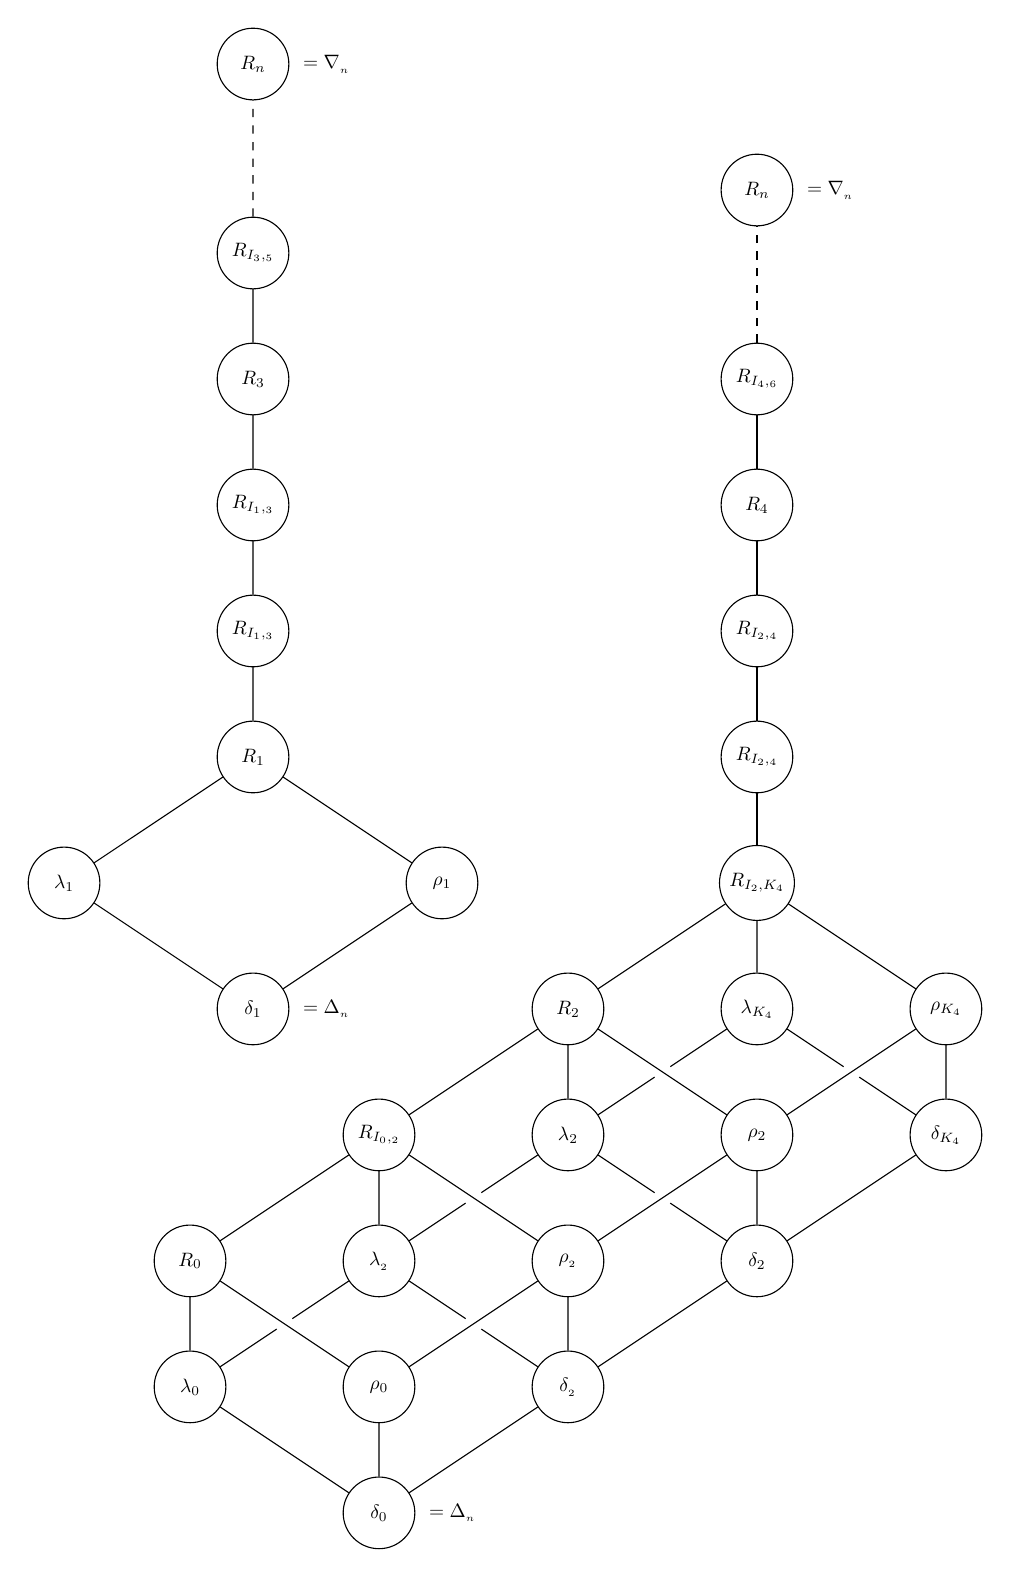
\begin{tikzpicture}
    [cong/.style={circle, minimum size=1.3cm, draw},
    scale=0.8, every node/.style={scale=0.7}]
    \node[cong] (Rn)  at ( 0,19) {$R_n$};
    \node[cong] (RA6) at ( 0,16) {$R_{I_4,\Alt_6}$};
    \node[cong] (R4)  at ( 0,14) {$R_4$};
    \node[cong] (RS4) at ( 0,12) {$R_{I_2,\Sym_4}$};
    \node[cong] (RA4) at ( 0,10) {$R_{I_2,\Alt_4}$};

    \node[cong] (RK)  at ( 0, 8) {$R_{I_2,K_4}$};
    \node[cong] (rK)  at ( 3, 6) {$\rho_{K_4}$};
    \node[cong] (lK)  at ( 0, 6) {$\lambda_{K_4}$};
    \node[cong] (dK)  at ( 3, 4) {$\delta_{K_4}$};

    \node[cong] (R2)  at (-3, 6) {$R_2$};
    \node[cong] (r2)  at ( 0, 4) {$\rho_2$};
    \node[cong] (l2)  at (-3, 4) {$\lambda_2$};
    \node[cong] (d2)  at ( 0, 2) {$\delta_2$};

    \node[cong] (RS2) at (-6, 4) {$R_{I_0,\Sym_2}$};
    \node[cong] (rS2) at (-3, 2) {$\rho_{\Sym_2}$};
    \node[cong] (lS2) at (-6, 2) {$\lambda_{\Sym_2}$};
    \node[cong] (dS2) at (-3, 0) {$\delta_{\Sym_2}$};

    \node[cong] (R0)  at (-9, 2) {$R_0$};
    \node[cong] (r0)  at (-6, 0) {$\rho_0$};
    \node[cong] (l0)  at (-9, 0) {$\lambda_0$};
    \node[cong] (d0)  at (-6,-2) {$\delta_0$};

    \node at ( 1.17, 19) {$=\nabla_{\Brau_n}$};
    \node at (-4.83, -2) {$=\Delta_{\Brau_n}$};

    % Bottom layer 
    \draw (d0)--(l0) (dS2)--(lS2) (d2)--(l2) (dK)--(lK);
    \draw (d0)--(dS2)--(d2)--(dK);
    \draw (l0)--(lS2)--(l2)--(lK);

    % Crossovers
    \fill[white] (-4.5,1)circle(.15) (-7.5,1)circle(.15);
    \fill[white] (-1.5,3)circle(.15) (-4.5,3)circle(.15);
    \fill[white] ( 1.5,5)circle(.15) (-1.5,5)circle(.15);

    % Supports
    \draw (d0)--(r0) (dS2)--(rS2) (d2)--(r2) (dK)--(rK);
    \draw (l0)--(R0) (lS2)--(RS2) (l2)--(R2) (lK)--(RK);
    
    % Top layer 
    \draw (r0)--(R0) (rS2)--(RS2) (r2)--(R2) (rK)--(RK);
    \draw (r0)--(rS2)--(r2)--(rK);
    \draw (R0)--(RS2)--(R2)--(RK);

    % Wick
    \draw (RK)--(RA4)--(RS4)--(R4)--(RA6);
    \draw[dashed] (RA6)--(Rn);

    % Odd
    \node[cong] (Rno) at (- 8,21) {$R_n$};
    \node[cong] (RA5) at (- 8,18) {$R_{I_3,\Alt_5}$};
    \node[cong] (R3)  at (- 8,16) {$R_3$};
    \node[cong] (RS3) at (- 8,14) {$R_{I_1,\Sym_3}$};
    \node[cong] (RA3) at (- 8,12) {$R_{I_1,\Alt_3}$};
    \node[cong] (R1)  at (- 8,10) {$R_1$};
    \node[cong] (l1)  at (-11, 8) {$\lambda_1$};
    \node[cong] (r1)  at (- 5, 8) {$\rho_1$};
    \node[cong] (d1)  at (- 8, 6) {$\delta_1$};
    \node at (-6.83, 21) {$=\nabla_{\Brau_n}$};
    \node at (-6.83,  6) {$=\Delta_{\Brau_n}$};
    \draw (d1)--(l1)--(R1)--(r1)--(d1);
    \draw (R1)--(RA3)--(RS3)--(R3)--(RA5);
    \draw[dashed] (RA5)--(Rno);
  \end{tikzpicture}
  \caption[Congruence lattice of $\Brau_n$]{Congruence lattice of $\Brau_n$ when
    $n$ is odd (upper left) and even (lower right)}
  \label{fig:bn-congs}
\end{figure}

\subsubsection{Jones monoid $\Jon_n$}
\nomenclature[Jn]{$\Jon_n$}{Jones monoid}
\index{Jones monoid}

The Jones monoid $\Jon_n$ is the submonoid of $\Prt_n$ consisting of all planar
bipartitions with blocks of size $2$.  By this definition, we can see that
$\Jon_n = \PP_n \cap \Brau_n$.  Its size is given by the Catalan number $C_n$
\citeoeis{A000108}.

As with the Brauer monoid, we consider two different cases based on whether $n$
is odd or even; however, the congruence lattices are much simpler.  If $n$ is
odd, then the only congruences are $\delta_1$, $\lambda_1$, $\rho_1$, and the
Rees congruences $\{R_1, R_3, \ldots, R_n\}$.  If, on the other hand, $n$ is even,
then the congruence lattice is isomorphic to that of $\Mot_{n/2}$, and its
description can be obtained by doubling each number in the description of that
lattice.  That is, the congruences are precisely
$$\{\delta_0, \delta_2, \lambda_0, \lambda_2, \rho_0, \rho_2, R_0, R_2, \ldots,
R_n\}.$$
These results are proven in \cite[\S9]{ourpaper}, and the lattices are shown in
Figure \ref{fig:jn-congs}.

\begin{figure}[ht]
  \centering
  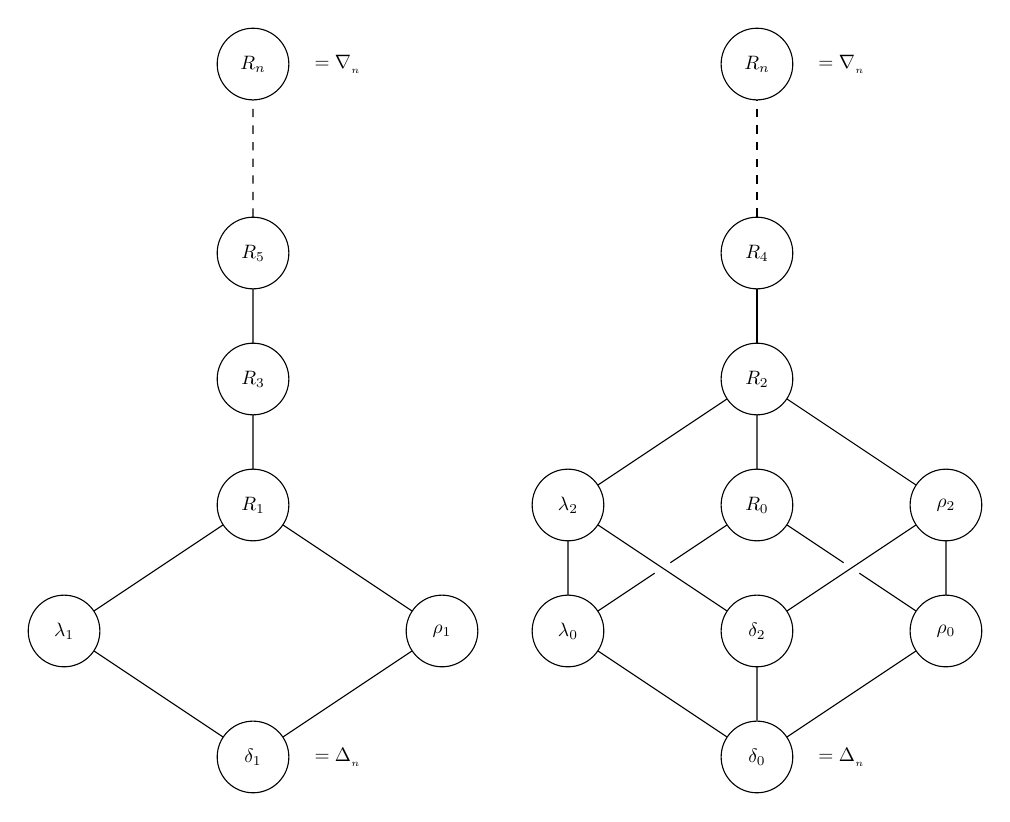
\begin{tikzpicture}
    [cong/.style={circle, minimum size=1.3cm, draw},
    scale=0.8, every node/.style={scale=0.7}]

    % Even
    \node[cong] (Rn) at ( 0,13) {$R_n$};
    \node[cong] (R4) at ( 0,10) {$R_4$};
    \node[cong] (R2) at ( 0, 8) {$R_2$};
    \node[cong] (l2) at (-3, 6) {$\lambda_2$};
    \node[cong] (R0) at ( 0, 6) {$R_0$};
    \node[cong] (r2) at ( 3, 6) {$\rho_2$};
    \node[cong] (l0) at (-3, 4) {$\lambda_0$};
    \node[cong] (d2) at ( 0, 4) {$\delta_2$};
    \node[cong] (r0) at ( 3, 4) {$\rho_0$};
    \node[cong] (d0) at ( 0, 2) {$\delta_0$};
    \node at (1.35,13) {$=\nabla_{\Jon_n}$};
    \node at (1.35, 2) {$=\Delta_{\Jon_n}$};
    \draw (d0)--(l0) (d0)--(r0) (l0)--(R0) (r0)--(R0);
    \fill[white] (-1.5,5)circle(.15) (+1.5,5)circle(.15);
    \draw (d0)--(d2) (l0)--(l2) (r0)--(r2) (R0)--(R2);
    \draw (d2)--(l2) (d2)--(r2) (l2)--(R2) (r2)--(R2);
    \draw (R2)--(R4);
    \draw[dashed] (R4)--(Rn);

    % Odd
    \node[cong] (Rno) at (- 8,13) {$R_n$};
    \node[cong] (R5)  at (- 8,10) {$R_5$};
    \node[cong] (R3)  at (- 8, 8) {$R_3$};
    \node[cong] (R1)  at (- 8, 6) {$R_1$};
    \node[cong] (l1)  at (-11, 4) {$\lambda_1$};
    \node[cong] (r1)  at (- 5, 4) {$\rho_1$};
    \node[cong] (d1)  at (- 8, 2) {$\delta_1$};
    \node at (-6.65, 13) {$=\nabla_{\Jon_n}$};
    \node at (-6.65,  2) {$=\Delta_{\Jon_n}$};
    \draw (d1)--(l1)--(R1)--(r1)--(d1);
    \draw (R1)--(R3)--(R5);
    \draw[dashed] (R5)--(Rno);
  \end{tikzpicture}
  \caption[Congruence lattice of $\Jon_n$]{Congruence lattice of $\Jon_n$ when
    $n$ is odd (left) and even (right)}
  \label{fig:jn-congs}
\end{figure}

\subsubsection{Bipartition monoid $\Prt_n$ and partial Brauer monoid $\PB_n$}
\index{partial Brauer monoid}
\nomenclature[PBn]{$\PB_n$}{Partial Brauer monoid}

Finally, we can state the congruence lattice of the entire bipartition monoid
$\Prt_n$.  As in the case of the Motzkin monoid, we have Rees congruences
$\{R_0, R_1, \ldots, R_n\}$ and lifted congruences
$\{\delta_0, \delta_1, \lambda_0, \lambda_1, \rho_0, \rho_1\}$.  The additional
congruences on $\Prt_n$ come from IN-pairs: the retractable IN-pair
$(I_1, \Sym_2)$ gives rise to congruences
$$\delta_{\Sym_2} = \zeta_{I_1,\Sym_2,\Delta},\quad
\lambda_{\Sym_2} = \zeta_{I_1,\Sym_2,\lL^{I_0}},\quad
\rho_{\Sym_2} = \zeta_{I_1,\Sym_2,\rR^{I_0}},\quad
R_{I_1,\Sym_2};$$
and the non-retractable IN-pairs $(I_{k-1},\Alt_k)$ and $(I_{k-1},\Sym_k)$ give
us the congruences $R_{I_{k-1},\Alt_k}$ and $R_{I_{k-1},\Alt_k}$, for
$k \in \{3, \ldots, n\}$.  Uniquely for $k=4$ we also have the IN-pair
$(I_3, K_4)$, yielding the congruence $R_{I_3,K_4}$.  These are all the
congruences on $\Prt_n$, as is proven in \cite[\S5]{ourpaper}.  The lattice is
shown in Figure \ref{fig:pn-congs}.

We should also mention the partial Brauer monoid $\PB_n$, the submonoid of
$\Prt_n$ consisting of all the bipartitions with blocks of size $1$ or $2$.  It
has $$\sum_{k=0}^n \binom{2n}{2k} (2k-1)!!$$ elements \citeoeis{A066223}, as
shown in \cite[2.1]{halverson_2014}.  Its congruence lattice has the same
description as that of $\Prt_n$ \cite[\S6]{ourpaper}, and is therefore also
shown in Figure \ref{fig:pn-congs}.

\begin{figure}[p]
  \centering
  \begin{tikzpicture}
    [cong/.style={circle, minimum size=1.3cm, draw},
    scale=0.8, every node/.style={scale=0.7}]
    \node[cong] (Rn)  at ( 0,17) {$R_n$};
    \node[cong] (R3)  at ( 0,14) {$R_3$};
    \node[cong] (RS3) at ( 0,12) {$R_{I_2,\Sym_3}$};
    \node[cong] (RA3) at ( 0,10) {$R_{I_2,\Alt_3}$};
    \node[cong] (R2)  at ( 0, 8) {$R_2$};

    \node[cong] (RS2) at ( 0, 6) {$R_{I_1,\Sym_2}$};
    \node[cong] (rS2) at ( 3, 4) {$\rho_{\Sym_2}$};
    \node[cong] (lS2) at ( 0, 4) {$\lambda_{\Sym_2}$};
    \node[cong] (dS2) at ( 3, 2) {$\delta_{\Sym_2}$};

    \node[cong] (R1)  at (-3, 4) {$R_1$};
    \node[cong] (r1)  at ( 0, 2) {$\rho_1$};
    \node[cong] (l1)  at (-3, 2) {$\lambda_1$};
    \node[cong] (d1)  at ( 0, 0) {$\delta_1$};

    \node[cong] (R0)  at (-6, 2) {$R_0$};
    \node[cong] (r0)  at (-3, 0) {$\rho_0$};
    \node[cong] (l0)  at (-6, 0) {$\lambda_0$};
    \node[cong] (d0)  at (-3,-2) {$\delta_0$};

    \node at ( 1.17, 17) {$=\nabla_{\Prt_n}$};
    \node at (-1.83, -2) {$=\Delta_{\Prt_n}$};

    % Bottom layer 
    \draw (d0)--(l0) (d1)--(l1) (dS2)--(lS2);
    \draw (d0)--(d1)--(dS2);
    \draw (l0)--(l1)--(lS2);

    % Crossovers
    \fill[white] (-4.5,1)circle(.15) (-1.5,1)circle(.15);
    \fill[white] (-1.5,3)circle(.15) ( 1.5,3)circle(.15);

    % Supports
    \draw (d0)--(r0) (d1)--(r1) (dS2)--(rS2);
    \draw (l0)--(R0) (l1)--(R1) (lS2)--(RS2);
    
    % Top layer 
    \draw (r0)--(R0) (r1)--(R1) (rS2)--(RS2);
    \draw (r0)--(r1)--(rS2);
    \draw (R0)--(R1)--(RS2);

    % Wick
    \draw (RS2)--(R2)--(RA3)--(RS3)--(R3);
    \draw[dashed] (R3)--(Rn);
  \end{tikzpicture}
  \caption{Congruence lattice of $\Prt_n$ (or $\PB_n$)}
  \label{fig:pn-congs}
\end{figure}
